%%%%%%%%%%%%%% 
% Fichero: EjBibtex
% Autor: J. Salido (http://www.esi.uclm.es/www/jsalido)
% Fecha: febrero, 2017
% Descripción: Gestión de bibliografía con BibTeX
% Ejemplo del curso: “LaTeX esencial para preparación de TFG, Tesis
% y otros documentos académicos” (Esc. Sup. Informática-UCLM)
%%%%%%%%%%%%%%




% -------------------------
%
% PREÁMBULO
% BEGIN_FOLD
% -------------------------

\documentclass[ 		% Clase del documento
	11pt,				% Tamaño de letra
	a4paper,			% Tamaño de papel
	twoside,			% Impresión a doble cara
	openright,			% La apertura de cap. a la dcha.
%	draft       		% Versión borrador (sin figuras)
	final       		% Versión final
]{book}
 
\usepackage[spanish,es-tabla, es-noindentfirst]{babel} % Internacionalización

%--- Márgenes del documento
\usepackage[top=2.5cm,bottom=2.5cm,inner=3.5cm,outer=2cm]{geometry}
\usepackage[skip=.3\baselineskip plus 2pt,indent]{parskip} % Salto entre párrafos 
% skip= .5\baselineskip plus 2pt -> Valor por defecto
% 

\usepackage{amsmath,amssymb,amsfonts} % Para ecuaciones
\usepackage{siunitx}
\usepackage{cancel}
\usepackage[normalem]{ulem}

%--- Si no se emplea ningún paquete de tipografía se emplea Computern Modern.
% -------------------------
% AJUSTE DE TIPOGRAFÍA (paquete específico para cada tipografía)
% -------------------------
%--- (Opción: Latin Modern)
%\usepackage{lmodern} % Latin Modern. Sucesora de Computer Modern.

%--- (Opción: Libertine)
%\usepackage[tt=false]{libertine} % Libertine con Old-Style Figures [osf]
%\usepackage[libertine]{newtxmath} % Times

%--- (Opción: Palatino)
%\usepackage{newpxtext} % Palatino: La opción osf proporciona números en old style.
%\usepackage{newpxmath}	% Palatino

%--- (Opción: Fourier)
\usepackage{fourier}   % Utopía
%---

\usepackage{textcomp,marvosym,pifont,fontawesome5} % Símbolos especiales
\usepackage[T1]{fontenc}% Codificación de salida    

\usepackage[shortlabels]{enumitem} 	% Control de listas
\usepackage{multicol}	% Texto en varias columnas

\usepackage{array,booktabs,tabularx,multirow}   % Paquetes para tablas
\usepackage{graphicx,subcaption,rotating,float} % Inclusión de figuras y subfiguras
\DeclareGraphicsExtensions{.pdf,.png,.jpg} % Precedencia de extensiones
\graphicspath{{./figs/}}% Path de búsqueda de ficheros gráficos

\usepackage[% Personalización de títulos de figuras y tablas
	margin=10pt,		% Margen
	font=small,			% Tamaño de tipografía
	labelfont=bf,		% Prefijo-Etiqueta en negrita
	format=hang			%
]{caption}
% -------------------------
% AJUSTE DE TÍTULOS (paquete caption)
% -------------------------
\captionsetup[table]{skip=5pt} 	% Separación de título tablas
\captionsetup[figure]{skip=5pt} % Separación de título en figuras
% -------------------------

\usepackage[usenames,dvipsnames,svgnames,x11names,table]{xcolor}
% -------------------------
% AJUSTE DE COLORES (paquete xcolor)
% -------------------------
\definecolor{palered}{rgb}{0.78, 0.03, 0.08}
\definecolor{ocre}{RGB}{243,102,25} % Ocre
\definecolor{aquaESI}{RGB}{0,151,215} % Aqua
\definecolor{turquesa}{RGB}{64,132,64} % Turquesa
\definecolor{UCLMred}{cmyk}{0.19, 1.0, 0.74, 0.12} % Color imagen corporativa UCLM
\definecolor{sombra}{HTML}{F0F0F0} % Sombra código
\definecolor{gris}{gray}{0.4} % Gris numeración código
% -------------------------

% -------------------------
% AJUSTE DE HIPERENLACES (paquete hyperref)
% -------------------------
\usepackage[pdftex,
	breaklinks=true,			% Permite que los enlaces ocupen más de una línea
]{hyperref}
\urlstyle{sf}			% Estilo sans serif para URLs
\pdfoptionpdfminorversion=6

\hypersetup{% (Metadatos del fichero PDF generado)
    linktocpage=true,        % true = enlace al nº de pág., false=texto completo
	colorlinks=true,         % true=colorea texto del enlace, false=recuadra el texto
%    hidelinks,               % Oculta colores en los enlaces (en negro)
    linkcolor=UCLMred,       % Color links internos
    anchorcolor=UCLMred,     % Color para anclas a texto
	urlcolor=aquaESI,        % Color para URL enlazadas
	citecolor=UCLMred,       % Color para citas a bibliografía
	bookmarksopen=true,      % Abre PDF con panel de marcadores abierto
	bookmarksnumbered=true,  % Incluye números en marcadores
	pdftoolbar=true,         % Muestra la toolbar de Acrobat
	pdfmenubar=true,	     % Muestra la menubar de Acrobat
}
% -------------------------

\usepackage{pdfpages}   % Permite inclusión de páginas de un PDF
\usepackage{microtype}  % Mejoras de microtipografía (solo pdflatex)

\usepackage{tikz}       % Paquete para gráficos
\usepackage[
	type={CC},
	modifier={by-sa},
	version={4.0},
]{doclicense}


\usepackage[lined,boxruled,algochapter,commentsnumbered,spanish]{algorithm2e} 

\usepackage{listings}	% Inclusión de listados de código
% -------------------------
% CONFIGURACIÓN LISTADOS DE CÓDIGO (paquete listings)
% -------------------------
\lstset{inputencoding=utf8, extendedchars=true,
	literate=%
	{á}{{\'a}}1 {é}{{\'e}}1 {í}{{\'i}}1 {ó}{{\'o}}1 {ú}{{\'u}}1
	{Á}{{\'A}}1 {É}{{\'E}}1 {Í}{{\'I}}1 {Ó}{{\'O}}1 {Ú}{{\'U}}1
	{à}{{\`a}}1 {è}{{\`e}}1 {ì}{{\`i}}1 {ò}{{\`o}}1 {ù}{{\`u}}1
	{À}{{\`A}}1 {È}{{\'E}}1 {Ì}{{\`I}}1 {Ò}{{\`O}}1 {Ù}{{\`U}}1
	{ä}{{\"a}}1 {ë}{{\"e}}1 {ï}{{\"i}}1 {ö}{{\"o}}1 {ü}{{\"u}}1
	{Ä}{{\"A}}1 {Ë}{{\"E}}1 {Ï}{{\"I}}1 {Ö}{{\"O}}1 {Ü}{{\"U}}1
	{â}{{\^a}}1 {ê}{{\^e}}1 {î}{{\^i}}1 {ô}{{\^o}}1 {û}{{\^u}}1
	{Â}{{\^A}}1 {Ê}{{\^E}}1 {Î}{{\^I}}1 {Ô}{{\^O}}1 {Û}{{\^U}}1
	{œ}{{\oe}}1 {Œ}{{\OE}}1 {æ}{{\ae}}1 {Æ}{{\AE}}1 {ß}{{\ss}}1
	{ű}{{\H{u}}}1 {Ű}{{\H{U}}}1 {ő}{{\H{o}}}1 {Ő}{{\H{O}}}1
	{ç}{{\c c}}1 {Ç}{{\c C}}1 {ø}{{\o}}1 {å}{{\r a}}1 {Å}{{\r A}}1
	{€}{{\euro}}1 {£}{{\pounds}}1 {«}{{\guillemotleft}}1
	{»}{{\guillemotright}}1 {ñ}{{\~n}}1 {Ñ}{{\~N}}1 {¿}{{?`}}1
	{¡}{{\textexclamdown}}1
}

\lstset{ % Estilo por defecto
	belowcaptionskip=5pt, % Espacio bajo el título
	basicstyle={\footnotesize\ttfamily}, % Estilo básico para el texto
	%stringstyle=\textsl,        % Estilo para las cadenas
	stringstyle={\color{Green4}},
	commentstyle={\color{Green4}},% Estilo para los comentarios
	keywordstyle={\color{Blue1}},% Estilo para las palabras clave
	%	deletekeywords={}, 			% Quita keywords separadas por comas
	captionpos=t,               % Ajusta la posición de títulos 
	numbers=left,               % Posición de números de línea
	numberstyle={\color{gris}\tiny\sffamily},          % Tamaño del número de línea
	numberfirstline=false,
	firstnumber=1, 				%  Nº de la primera línea
	stepnumber=1,               % Paso de línea numerada
	numbersep=10pt,             % Separación del texto al número de línea
	tabsize=2,                  % Tamaño del tabulador
	texcl=true,				    % Necesario para unicode en los comentarios
	breaklines=true,            % Ajusta división automática de líneas
	breakatwhitespace=true,     % Indica si la división automática sólo ocurre en los espacios en blanco
	frame=none,               % none, leftline, topline, bottomline, lines, single, shadowbox 
%	frameround=tttt, 			% Redondea los bordes del frame
%	rulecolor={\color{black}},  % Color del frame
	showspaces=false,           % Muestra espacios en blanco
	showtabs=false,             % Muestra tabuladores
	showstringspaces=true,      % Muestra espacios en blanco en las cadenas        
	xleftmargin=1cm,xrightmargin=1cm,
	breaklines=true,
	postbreak=\mbox{\textcolor{red}{$\hookrightarrow$}\space}, % Flecha al saltar de linea
	prebreak=\mbox{\textcolor{red}{$\hookleftarrow$}\space}, % Flecha al saltar de linea	
    framexleftmargin=8mm, % Ajuste para que el nº de línea quede dentro del frame
	%	framexrightmargin=5pt,
	%	framexbottommargin=4pt,
	backgroundcolor={\color{sombra}} % Color del fondo
}

\lstdefinestyle{consola}{% Estilo para comandos tipo consola
	basicstyle={\color{white}\scriptsize\bf\ttfamily},
	backgroundcolor={\color{black}},
	frame=none,
	showspaces=true
}

\lstdefinestyle{ruled}{% Estilo para listado con filete a la izda.
	frame=L,
	rulesep=.1pt,
   	framexleftmargin=0mm,
	rulecolor=\color{black}
}

% OJO: Definición de dos macros para el tratamiento correcto de comentarios con % en Matlab
% (sólo necesario si se desea incluir código Matlab)
\makeatletter
\def\spanishplainpercent{\let\es@sppercent\@empty}
\def\spanishpercent{\def\es@sppercent{\unskip\textormath{$\m@th\,$}{\,}}}
\makeatother

% -------------------------
%--- OPT.: Paquete para incluir menús, paths y teclas de modo "elegante"
\usepackage[os=win]{menukeys} 
% OJO: Este paquete presenta algunas incompatibilidades, debe cargarse el 
% último (manejar con cuidado).

% Estas definiciones permiten cambiar el estilo de los elementos. Si se desean otros estilos o su configuación es preciso recurrir a la documentación del paquete (no lo recomiendo).
\renewmenumacro{\menu}[:]{menus} % OPT.: default: menus
\renewmenumacro{\directory}[/]{pathswithblackfolder} % OPT.: default: paths
\renewmenumacro{\keys}[+]{shadowedroundedkeys} % OPT.: default: roundedkeys
%---

% Paquetes especiales para Química
\usepackage[version=3]{mhchem}
\usepackage{chemfig}


% -------------------------
% -------------------------
% -------------------------
% END_FOLD





% -------------------------
% -------------------------
% -------------------------
% COMANDOS DE USUARIO
% -------------------------
% -------------------------
% -------------------------
% BEGIN_FOLD
% -------------------------
% Ajustes para el idioma español.
% EDITAR: Sólo si es necesario.
% NOTA: Al cambiar de idioma las def. de títulos se reinician.
\newcommand{\setindexnames}{%
	\renewcommand{\lstlistingname}{Listado}
	\renewcommand{\lstlistlistingname}{Índice de listados}
	\SetAlgorithmName{Algoritmo}{Alg}{Índice de algoritmos}
	% Modififica las macros \algorithmcfname y \listalgoritmcfname
	\renewcommand{\appendixname}{Anexo}
	\renewcommand{\bibname}{Bibliografía}
	\renewcommand{\indexname}{Índice temático}
}


% -------------------------
% INDICACIÓN DE PULSACIÓN DE TECLA
% -------------------------
% Uso: \tecla{<key>}
\usetikzlibrary{shadows} % Necesario para poder crear nuevo comando de indicación de pulsación de tecla.
\newcommand*\tecla[1]{%  Para crear indicaciones de pulsación de teclas
  \tikz[baseline=(key.base)]
    \node[%
      draw,fill=white,
      drop shadow={shadow xshift=0.25ex,shadow yshift=-0.25ex,fill=black,opacity=0.75},
      rectangle,rounded corners=2pt,inner sep=1pt,line width=0.5pt,
      font=\scriptsize\sffamily
    ](key) {#1\strut}
  ;
}

% -------------------------
% -------------------------
% -------------------------
% END_FOLD
% -------------------------
% -------------------------
% -------------------------

\usepackage{makeidx}
\makeindex

\begin{document}
\frontmatter

\begin{titlepage}
    \pdfbookmark{Portada}{portada}
    \begin{center}
    	\LARGE
    	{\bfseries Universidad de Castilla-La Mancha\par}
    	Escuela Superior de Informática\par
    	\vspace{4cm}
    	{\huge\bfseries Ejemplo de documento con \\
                        Índice de contenido\par}
    	{\small \phantom{(Portada 5)}}
    	\vspace{3cm}
    	\par
    \end{center}
	\hfill\begin{minipage}{.5\linewidth}
		\normalsize
		trabajo realizado por\par
		\textsc{Jesús Salido}\par
        (Curso de \LaTeX{} para TFG)
	\end{minipage}
	\vfill
	\centering	\today
\end{titlepage}

\cleardoublepage
\setcounter{tocdepth}{1} % Suprime del índice los apdos. de nivel mayor
\phantomsection % Necesario con hyperref
\pdfbookmark[0]{Índice general}{idx_toc}% idx_toc.0 % Bookmark en PDF
\tableofcontents
\listoffigures
\listoftables


\mainmatter

\chapter{Fuentes tipográficas y símbolos}
\LaTeX{} genera su salida con los tipos \emph{Computer Modern} (\textbf{CM}) creados por D.~Knuth con ayuda del programa \textsc{metafont}. Por suerte \LaTeX{} está configurado en la actualidad para incorporar estas <<fuentes>>\index{fuente} en los ficheros PDF como una fuente \emph{Postscript}\index{Postscript} Tipo 1 (vectorial). Con las fuentes Tipo 1 se obtiene una calidad superior a la obtenida con las fuentes Tipo 3 o de mapa de bits (\textbf{PK}) que solo ofrecen máxima calidad a la escala para la que han sido creadas. Por suerte en la actualidad \LaTeX{} ofrece la posibilidad de incluir las fuentes estándar \emph{Postscript} de \textsf{Adobe} utilizando los paquetes apropiados. Así es muy claro alternar en un texto entre las tres familias disponibles: Roman (redonda), \textsf{Sans Serif (paloseco, sin serifa o sin adornos)} y \texttt{Teletype (teletipo o monoespaciada)}. Y por último unas MAYÚSCULAS MÁS \textsc{pequeñas llamadas versalitas}. Recuerda que no debes emplear \underline{subrayado} para \emph{enfatizar}. Aunque en algún documento (p.~ej.\ ejercicios) su uso tampoco es habitual.\index{enfatizado}

Por supuesto \LaTeX{} tiene en cuenta las particularidades de la tipografía en modo matemático como en: $f(x)=y^2$ y números $1,2,3,4,5,6,7,8,9$, o en modo texto: 0123456789.

$$g(x)=\int_{0}^{\infty}y^{3}dy$$

En \TeX{} y \LaTeX{} las palabras ``reservadas'' o <<comandos>> del lenguaje están precedidos por la barra inclinada o \emph{backslash} (`\textbackslash'). Otros caracteres especiales son: \# \$ \% \textasciicircum \& \_ \{ \} \~{}. Para escribir estos caracteres se emplean los comandos:\index{comandos}
\verb!\# \$ \% \textasciicircum \& \_ \{ \} \~!. Recuerda que con el comando \verb+\verb+ se puede generar texto que \LaTeX{} no procesa.\footnote{Emplearlo con precaución.}

\LaTeX{} también puede generar un conjunto muy amplio de símbolos especiales como el \EUR{} o \texteuro, \ding{45} y \Coffeecup. En los textos informáticos un carácter habitual es \verb+~+ empleado en las direcciones URL. Este carácter se puede generar de varias formas (\verb+~+, \~{}, $\sim$). Aunque empleando el paquete \texttt{url} la escritura de direcciones electrónicas se simplifica, por ejemplo:

\url{http://osl.ugr.es/CTAN/info/symbols/comprehensive/symbols-a4.pdf}

\noindent es la dirección URL de \emph{The Comprehensive \LaTeX{} Symbol List} de Scott Pakin (2009) donde se hace un repaso de todos los símbolos y caracteres que se pueden generar en \LaTeX{}.

Un gran conjunto de iconos empleados en los textos informáticos se pueden obtener mediante el uso de la tipografía \texttt{awesome5} (con el paquete fontawesome5),\index{awesome5} como por ejemplo: \faNodeJs, \faNode, \faGooglePlay, \faInternetExplorer, \faGithub, \faGit*, \faWhatsapp, etc.

Al componer documentos en español hay que tener en cuenta las peculiaridades de la tipografía\index{tipografía} española frente a la inglesa para hacer un uso correcto de los recursos ofrecidos por \LaTeX.














\chapter{Elaboración de listas}
Las listas se emplean cuando se desea enumerar una serie de características, objetos, etc. A continuación veremos algunos ejemplos de listas.

\noindent Ejemplo de entorno {\tt itemize}:\index{itemize}
\index{codigo@código}\index{codigo@código!fuente}
% Ejemplo: Lista con viñetas
% ============
\begin{itemize}
	\item peras
	\item manzanas
    \item 	limones
    \item 	naranjas
\end{itemize}

\noindent La misma lista cambiando la viñeta, gracias a paquete \texttt{enumitem}:
% Ejemplo: Lista con viñeta dingbat
% ============
\begin{itemize}[\ding{68}]
	\item peras
	\item manzanas
	\item limones
	\item naranjas
\end{itemize}


Las listas también se pueden anidar:\index{listas anidadas}
% Ejemplo: Lista anidada con balas
% ============
\begin{itemize}
	\item peras
	\begin{itemize}
		\item conferencia
		\item ercolina
    	\begin{itemize}
    		\item mini conferencia
    		\item extra ercolina
    	\end{itemize}
	\end{itemize}
	\item manzanas
	\begin{itemize}
		\item granny
		\item golden 
	\end{itemize}
	\item naranjas
\end{itemize}


\noindent Ejemplo de entorno {\tt itemize} en el que se sustituye el símbolo (\emph{bullet}) por defecto:

% Ejemplo:
% ============
\begin{itemize}
	\item[*] peras
	\item manzanas
	\item[\ding{170}] naranjas
\end{itemize}


Personalmente, pienso que \LaTeX{} proporciona demasiado espaciado en las listas. Con el paquete \texttt{enumitem}\index{enumitem} se puede compactar las listas. A continuación se muestra un ejemplo de entorno {\tt itemize} con opciones para cambiar el espaciado vertical entre ítems y cambio de viñeta por defecto (proporcionada por el paquete \texttt{enumitem}):

% Ejemplo:
% ============
\begin{itemize}[noitemsep]
	\item peras
	\item manzanas
	\item naranjas
\end{itemize}

\noindent Ejemplo de entorno {\tt enumerate} para listas numeradas:\index{enumerate}

% Ejemplo:
% ============
\begin{enumerate}
	\item peras
	\item manzanas
	\item naranjas
\end{enumerate}


\noindent Ejemplo de entorno {\tt enumerate} con cambio de numeración (letras minúsculas) y opción \texttt{noitemsep}\index{noitemsep|see{enumitem}} (proporcionada por el paquete \texttt{enumitem}) para listas numeradas:

% Ejemplo:
% ============
\begin{enumerate}[a.-,noitemsep]
	\item peras
	\item manzanas
	\item naranjas
\end{enumerate}

\noindent Este es otro ejemplo de línea compacta creada en varias columnas con ayuda de los paquetes \texttt{enumitem} y \texttt{multicol}:\index{multicol}
% Ejemplo:
% ============
\begin{multicols}{2} % El parámetro es el número de columnas de la lista
	\begin{enumerate}[i.,noitemsep]
		\item peras
		\item manzanas
		\item naranjas
		\item patatas
		\item calabazas
		\item fresas
	\end{enumerate}
\end{multicols}


\noindent Las listas incluso se pueden personalizar (aunque debería estar justificado el cambiar el estilo por defecto, haciéndolo con mucha prudencia):

% Ejemplo:
% ============
\begin{enumerate}[\ding{52},noitemsep] % Lista en la que se cambia el bullet por un símbolo dingbat
	\item peras
	\item[\ding{55}] manzanas
	\item naranjas
\end{enumerate}


\noindent Así también:

% Ejemplo:
% ============
\begin{dingautolist}{192} % Lista con símbolos sucesivos de la tabla dingbat
	\item peras
	\item manzanas
	\item naranjas
\end{dingautolist}


\noindent y por supuesto anidar:

% Ejemplo:
% ============
\begin{enumerate}
  \item Cítricos
  \begin{enumerate}
    \item Limón
    \item Naranja
  \end{enumerate}
  \item Legumbres
  \item Hortalizas \ldots
\end{enumerate}


\noindent Ejemplo de entorno {\tt description} para listas:

% Ejemplo:
% ============
\begin{description}[noitemsep]
	\item[Estupideces] no mejoran por ponerlas en una lista por bonita que esta sea. Aunque la mona se vista de seda, mona se queda.
	\item[Lucideces] sin embargo, pueden parecer hermosas en
	una lista.
\end{description}

\noindent El ejemplo anterior formateado de otro modo:

% Ejemplo:
% ============
\begin{description}[style=nextline]
	\item[Estupideces] no mejoran por ponerlas en una lista por bonita que esta sea. Aunque la mona se vista de seda, mona se queda.
	\item[Lucideces] sin embargo, pueden parecer hermosas en una lista.
\end{description}

\LaTeX{} permite una configuración más avanzada para presentar listas más sofisticadas, aunque la mayoría de las veces esto no es necesario, ya que es suficiente con las listas convencionales.











\chapter{Inclusión de figuras}
La inclusión de figuras y archivos de imagen en un documento elaborado con \LaTeX{} es muy sencilla y versátil (en la Fig.~\ref{fig:plazaCR} se muestra una fotografía en formato \texttt{.jpg} en color).\footnote{El título de la imagen también muestra cómo debe darse créditos al autor de la imagen si ésta no es de libre uso y tenemos permiso para usarla.} Hay que tener presente que el tipo de ficheros permitidos depende de si empleamos \texttt{latex} o \texttt{pdflatex},\footnote{En todo este curso asumimos que trabajaremos con \texttt{pdflatex} pues es más cómodo y siempre es posible utilizar la herramienta \texttt{epstopdf} para realizar la conversión de formatos.} ya que el primero sólo permite la inclusión de ficheros gráficos \texttt{.eps} mientras el segundo admite \texttt{.pdf}, \texttt{.png} y \texttt{.jpg}. Cuando la figura original presente un formato diferente a los mencionados, será preciso emplear algún programa para realizar la conversión apropiada. La inclusión de figuras requiere al menos el empleo del paquete \texttt{graphicx}\index{graphicx} con el que ya se pueden obtener resultados muy aceptables.

\begin{figure}[hbt] % Véase los tags de ubicación (h)ere, (b)ottom, (t)op 
	\centering % Fig. centrada en la página
% 	EDITAR: En caso de requerir que el título aparezca en la parte superior de la figura.
%	\caption[Ejemplo de foto en formato jpg]{La Plaza Mayor (cortesía de J.~Salido)} % Título y el título para la lista de figuras
	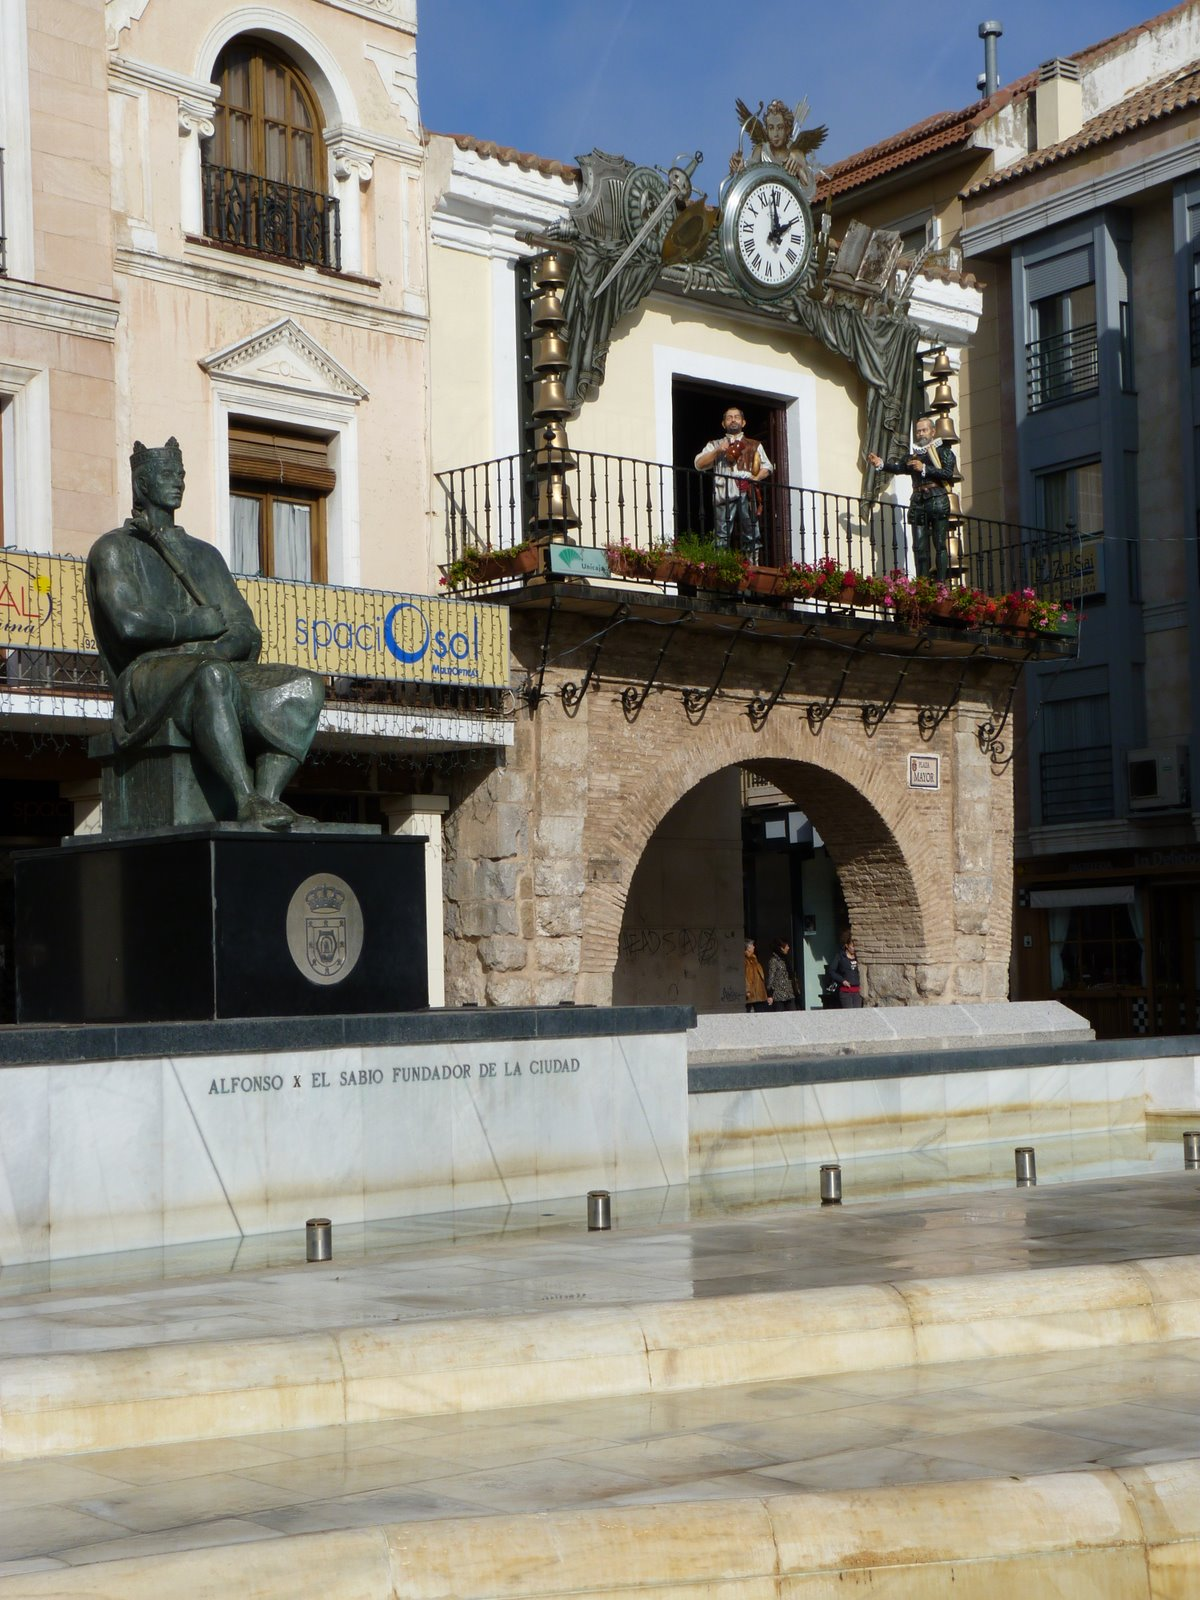
\includegraphics[height=8cm]{plazaCR} % Alto de la figura en la pág.
	\caption[Ejemplo de foto en formato jpg]{La Plaza Mayor (cortesía de J.~Salido).} % Título y el título para la lista de figuras
	\label{fig:plazaCR} % Etiqueta para las refs. cruzadas
\end{figure}

\LaTeX{} puede procesar las figuras como \emph{objetos deslizantes o <<flotantes>>}\footnote{Estos elementos se denominan \textit{float} y por ello a veces en español utilizamos como traducción <<flotante>>.} (o sin ubicación prefijada). De este modo \LaTeX{} emplea algoritmos para encontrar la mejor ubicación de todos los objetos flotantes que contenga el texto. El usuario siempre tiene a su disposición opciones para sugerir la ubicación deseada dejando a \LaTeX{} la reubicación del texto y párrafos en la página. Con todo, en ocasiones el usuario debe hacer algunos ajustes para conseguir la ubicación deseada, aunque sigue siendo un procedimiento mucho más cómodo que en algunos de los procesadores de texto populares de tipo \textsc{wysiwyg}. Siempre que existan muchas figuras en el texto, el ajuste del resultado final va a ser más complejo y requerirá mayor intervención humana.

Otra de las ventajas de \LaTeX{} es que las imágenes no están incrustadas en nuestro fichero fuente, sino que son ficheros independientes incluidos durante la compilación. De este modo, la modificación de la figura no requiere cambios del fichero fuente sino únicamente una nueva compilación.








\section{Formatos gráficos}
A la hora de incluir figuras se debe decidir qué formato\index{formatos gráficos} es el más apropiado siguiendo las siguientes reglas:
\begin{itemize}
	\item Siempre que sea posible es preferible el formato \texttt{.pfd}, ya que es vectorial (escalable) como el gráfico de la Fig.~\ref{fig:4004arch}. Por supuesto, si el fichero \textsf{PDF} contiene alguna imagen de mapa de bits, esta no será escalable.
	\item Las fotografías se incluirán en formato \texttt{.jpg} (como en las  Figs.~\ref{fig:mars} y \ref{fig:plazaCR}).
	\item Las capturas de pantalla o gráficos de gran contraste se deben incluir en formato \texttt{.png} (como en la Fig.~\ref{fig:inkscape}). 
	\item Siempre que se tenga un fichero de imagen (mapa de bits) con un fondo blanco u otro color plano, debería intentarse transformar en una imagen con fondo transparente convirtiéndola al formato \texttt{.png}.
\end{itemize}

\begin{figure}[hbt]
	\centering 
	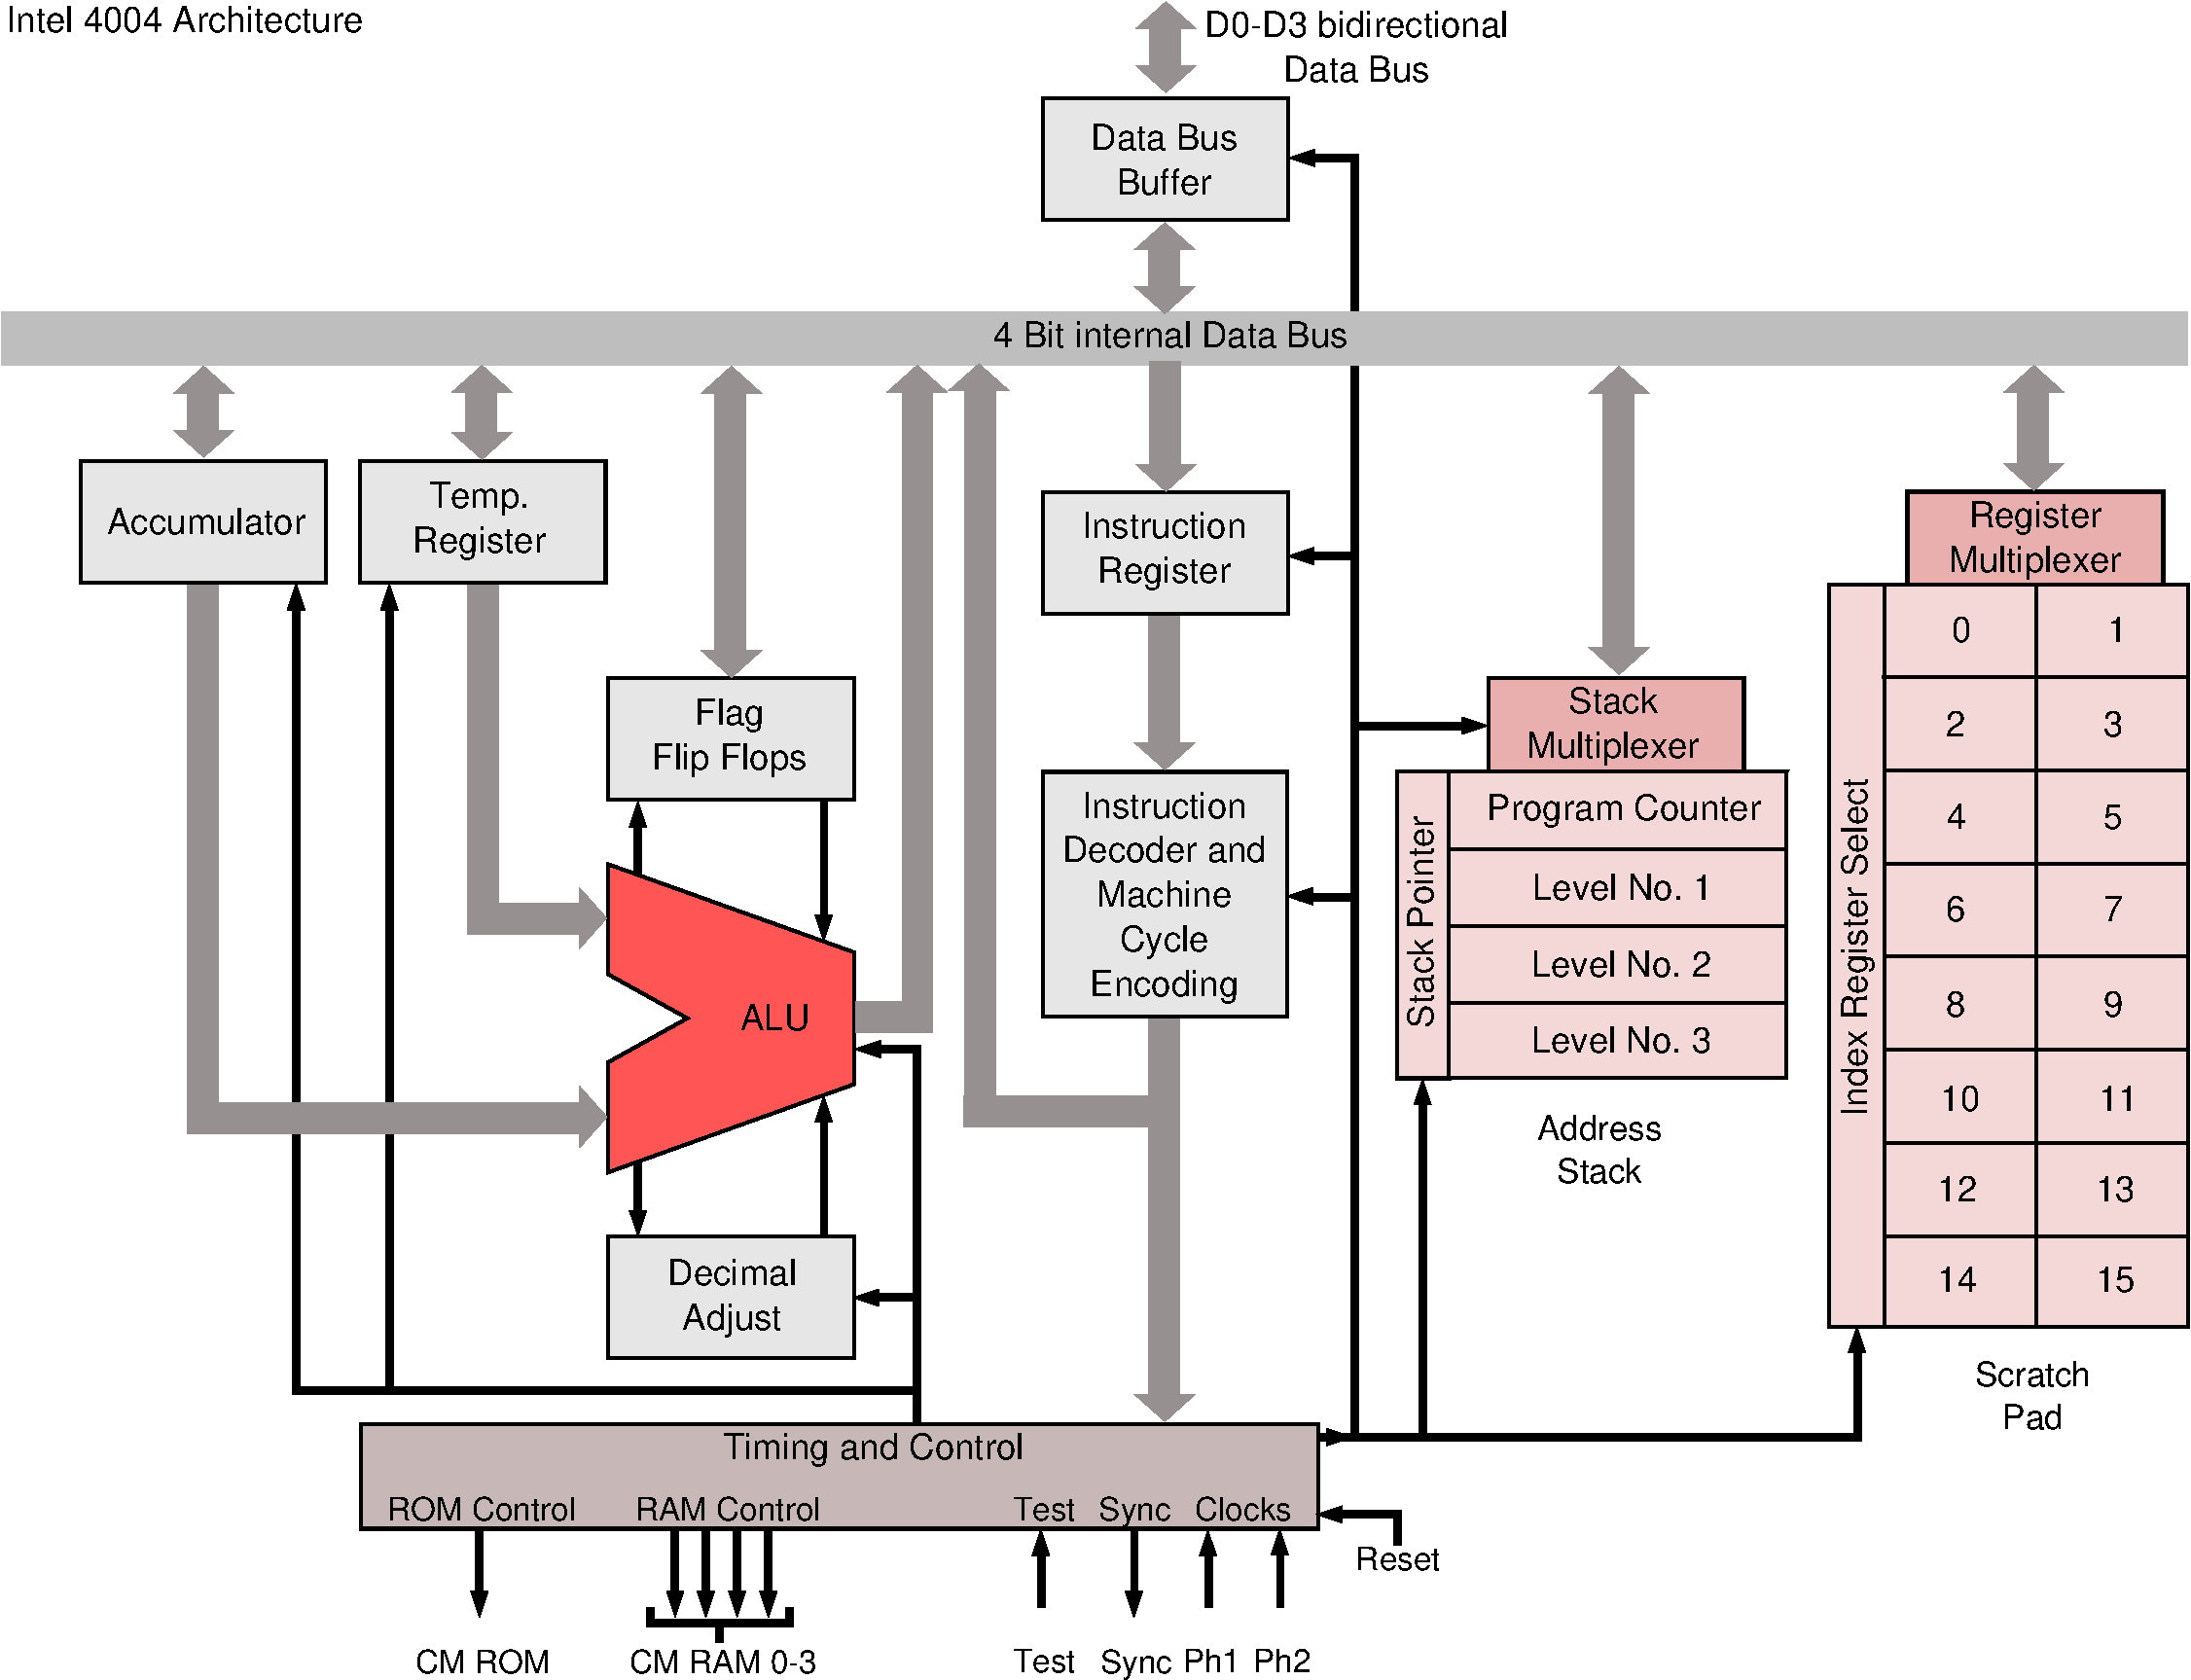
\includegraphics[width=0.8\textwidth]{4004arch} 
	\caption[Ejemplo de gráfico vectorial \textsf{PDF}]{Figura vectorial de arquitectura Intel 4004 en formato \textsf{PDF} (CC-BY-SA 3.0, Appaloosa, 2007. Wikimedia Commons).}
	\label{fig:4004arch}
\end{figure}

\begin{figure}[hbt]
	\centering
	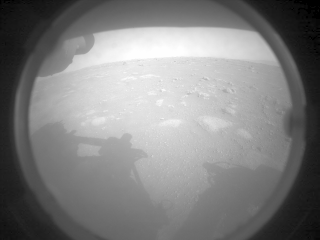
\includegraphics[width=0.5\textwidth]{Mars_Perseverance} 
	\caption[Foto histórica enviada desde Marte]{Primera foto enviada desde Marte el {18-2-2021} por el robot Perseverance incluida aquí en formato JPEG (cortesía de NASA/JPL-Caltech).}
	\label{fig:mars}
\end{figure}

\begin{figure}[H]
	\centering
	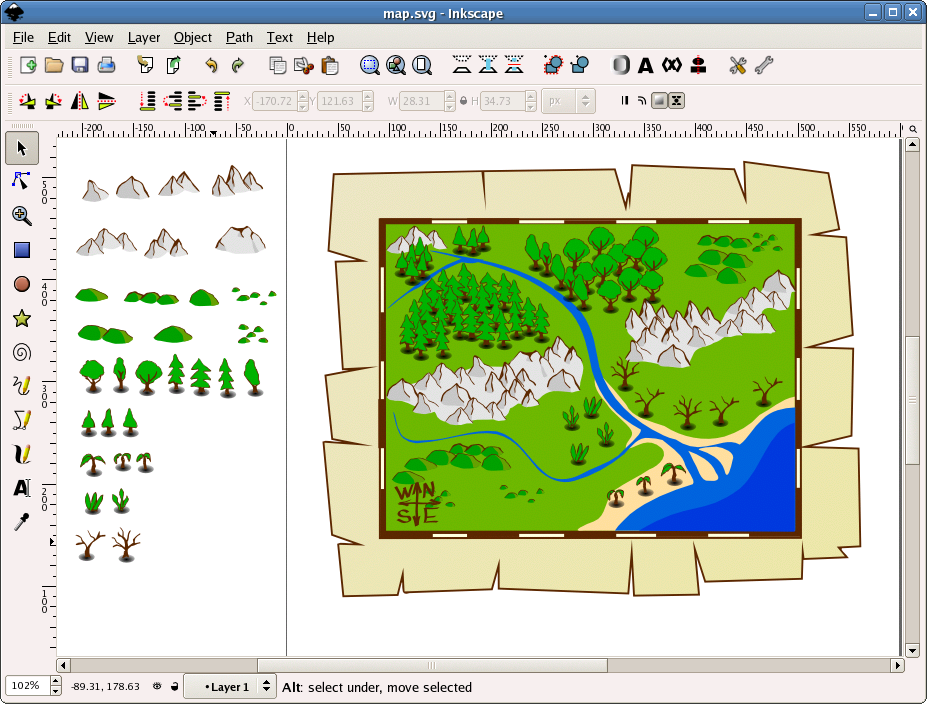
\includegraphics[width=0.7\textwidth]{inkscape} 
	\caption[Ejemplo de captura en png]{Captura de pantalla de \textsf{Inkscape} incluida en formato \textsf{PNG}.}
	\label{fig:inkscape}
\end{figure}



\section{Ventajas del formato \textsf{PDF}}
Una de las dificultades de trabajar con ficheros \textsf{PDF} es que se trata de un formato difícil de editar, de modo que habitualmente se genera a partir de otros formatos. Por ejemplo, el gráfico de la Fig.~\ref{fig:4004arch}, cuyo formato original es \textsf{SVG}, ha sido realizado con el programa \textsf{Inkscape} y convertido al formato \textsf{PDF} mediante la herramienta de exportación (a través de \textsf{Cairo}) incluida en el programa en dicho programa. En los programas que no incorporan dicha herramienta el fichero \textsf{PDF} se puede generar imprimiendo a un archivo con un driver de impresión \textsf{PDF}. 

Cuando se trabaja con figuras hay que tener mucho cuidado con emplear imágenes de Internet sin tener la seguridad de los términos de uso de las mismas. Con mucha frecuencia al utilizarlos, se violan los derechos de propiedad intelectual, incluso cometiendo involuntariamente un delito. Por este motivo recomiendo recurrir a librerías de dominio público y licencias\index{licencia de uso} de libre uso como Creative Commons\index{CC|see{licencias de uso}} ---permiten el uso de las imágenes y \emph{cliparts} con pocas restricciones--- como por ejemplo OpenClipArt,\footnote{\url{http://openclipart.org/}} la página de galerías en el sitio de Inkscape\footnote{\url{http://wiki.inkscape.org/wiki/index.php/Galleries}} y Wikimedia Commons.\footnote{\url{http://commons.wikimedia.org/}}\index{InkScape} El derecho a cita permite la reproducción de figuras, sujetas a derechos restrictivos de distribución, en ámbitos académicos. Sin embargo, siempre debería incluirse en el pie de la figura la atribución de autoría y la licencia que se aplica a la distribución de la misma (no confundir con la licencia de nuestro documento). En cualquier caso debería investigarse la licencia de uso de la figura puesto que en algunos casos (p.~ej.\ banco de imágenes de la \textsc{nasa}) el autor señala cómo debe realizarse la atribución de autoría. En ningún caso puede incluirse una figura ajena sin atribución, sin importar si es de dominio público o distribuida con una licencia permisiva.


\section{Gráficas matemáticas}
En muchas ocasiones es preciso recurrir a una gráfica matemática para reflejar o apoyar una idea. Existen numerosos programas que ayudan a realizar estas gráficas, en cualquiera de los casos siempre se empleará un formato vectorial (\textsf{PDF}) para incluir la gráfica en nuestro documento. Nunca debe hacerse mediante una captura de pantalla pues, en este caso estaremos perdiendo mucha información al tratar como un mapa de bits algo que es un objeto matemático y por tanto, independiente de su escala de representación.

Uno de los programas más universales para la creación de gráficas matemáticas son las hojas de cálculo como Excel.\index{Excel} La Fig.~\ref{fig:excel} muestra un ejemplo de figura vectorial generada con ayuda de dicho programa.

\begin{figure}[H]
	\centering
	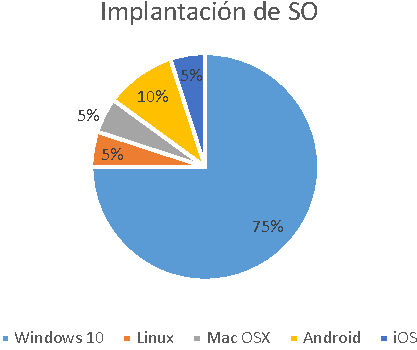
\includegraphics[width=0.5\textwidth]{EjFigsExcelOrig-crop} 
	\caption[Gráfico de Excel]{Figura vectorial generada con Excel.}
	\label{fig:excel}
\end{figure}

La Fig.~\ref{fig:matlabGrafs} muestra un ejemplo de figura vectorial generada con ayuda del programa Matlab.\index{Matlab} En este caso se observa cómo una única figura contiene distintos gráficos. 

\begin{figure}[H]
	\centering
	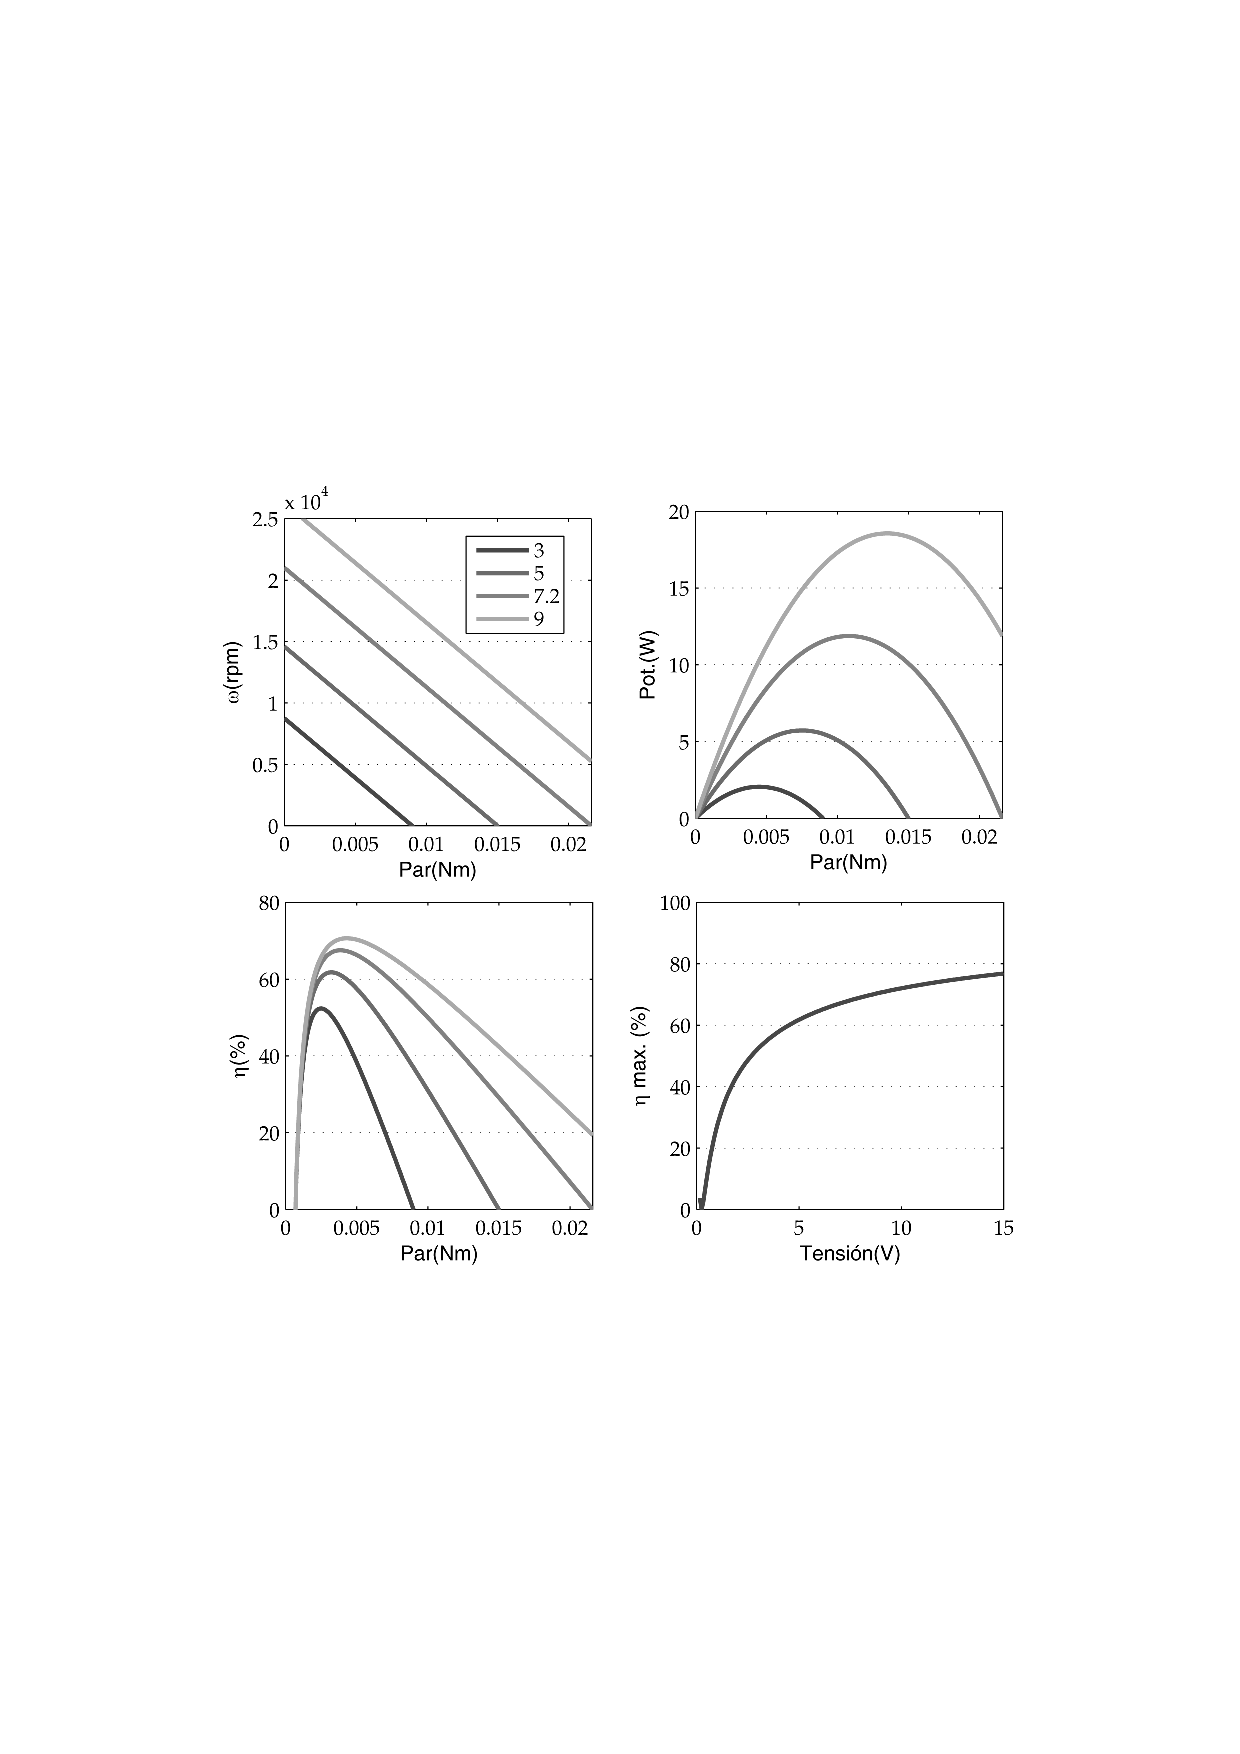
\includegraphics[width=0.8\textwidth]{matlabGrafs} 
	\caption[Gráfico de Matlab]{Figura vectorial generada con Matlab.}
	\label{fig:matlabGrafs}
\end{figure}




\section{Métodos avanzados de inclusión de figuras}
En esta sección se describen e ilustran métodos especializados y consejos para incluir gráficos en un documento \LaTeX.


\subsection{Subfiguras}
La inclusión de figuras requiere al menos el empleo del paquete \texttt{graphicx} con el que ya se pueden obtener resultados muy aceptables, aunque existen otros paquetes más especializados que facilitan hacer cosas más exóticas, como el paquete \texttt{subcaption}\index{subcaption} para presentar figuras compuestas de varias subfiguras\index{subfiguras} (ver ejemplos en las Figs.~\ref{fig:clock} y \ref{fig:lion}). A pesar de la posibilidad del uso del paquete \texttt{subcaption} no se debe descartar la alternativa de la composición externa a \LaTeX{} de las subfiguras y su inclusión en el documento como una figura sencilla como en la Fig.~\ref{fig:2clock}. Esta alternativa hace innecesario el empleo de paquetes dedicados.

\begin{figure}[hbt]
	\centering
	\begin{subfigure}[b]{0.48\textwidth}
		\centering
		\includegraphics[width=\textwidth]{clockCR}
		\caption{Imagen jpg en color}\label{fig:clockCR}
	\end{subfigure}
	\begin{subfigure}[b]{0.48\textwidth}
		\centering
		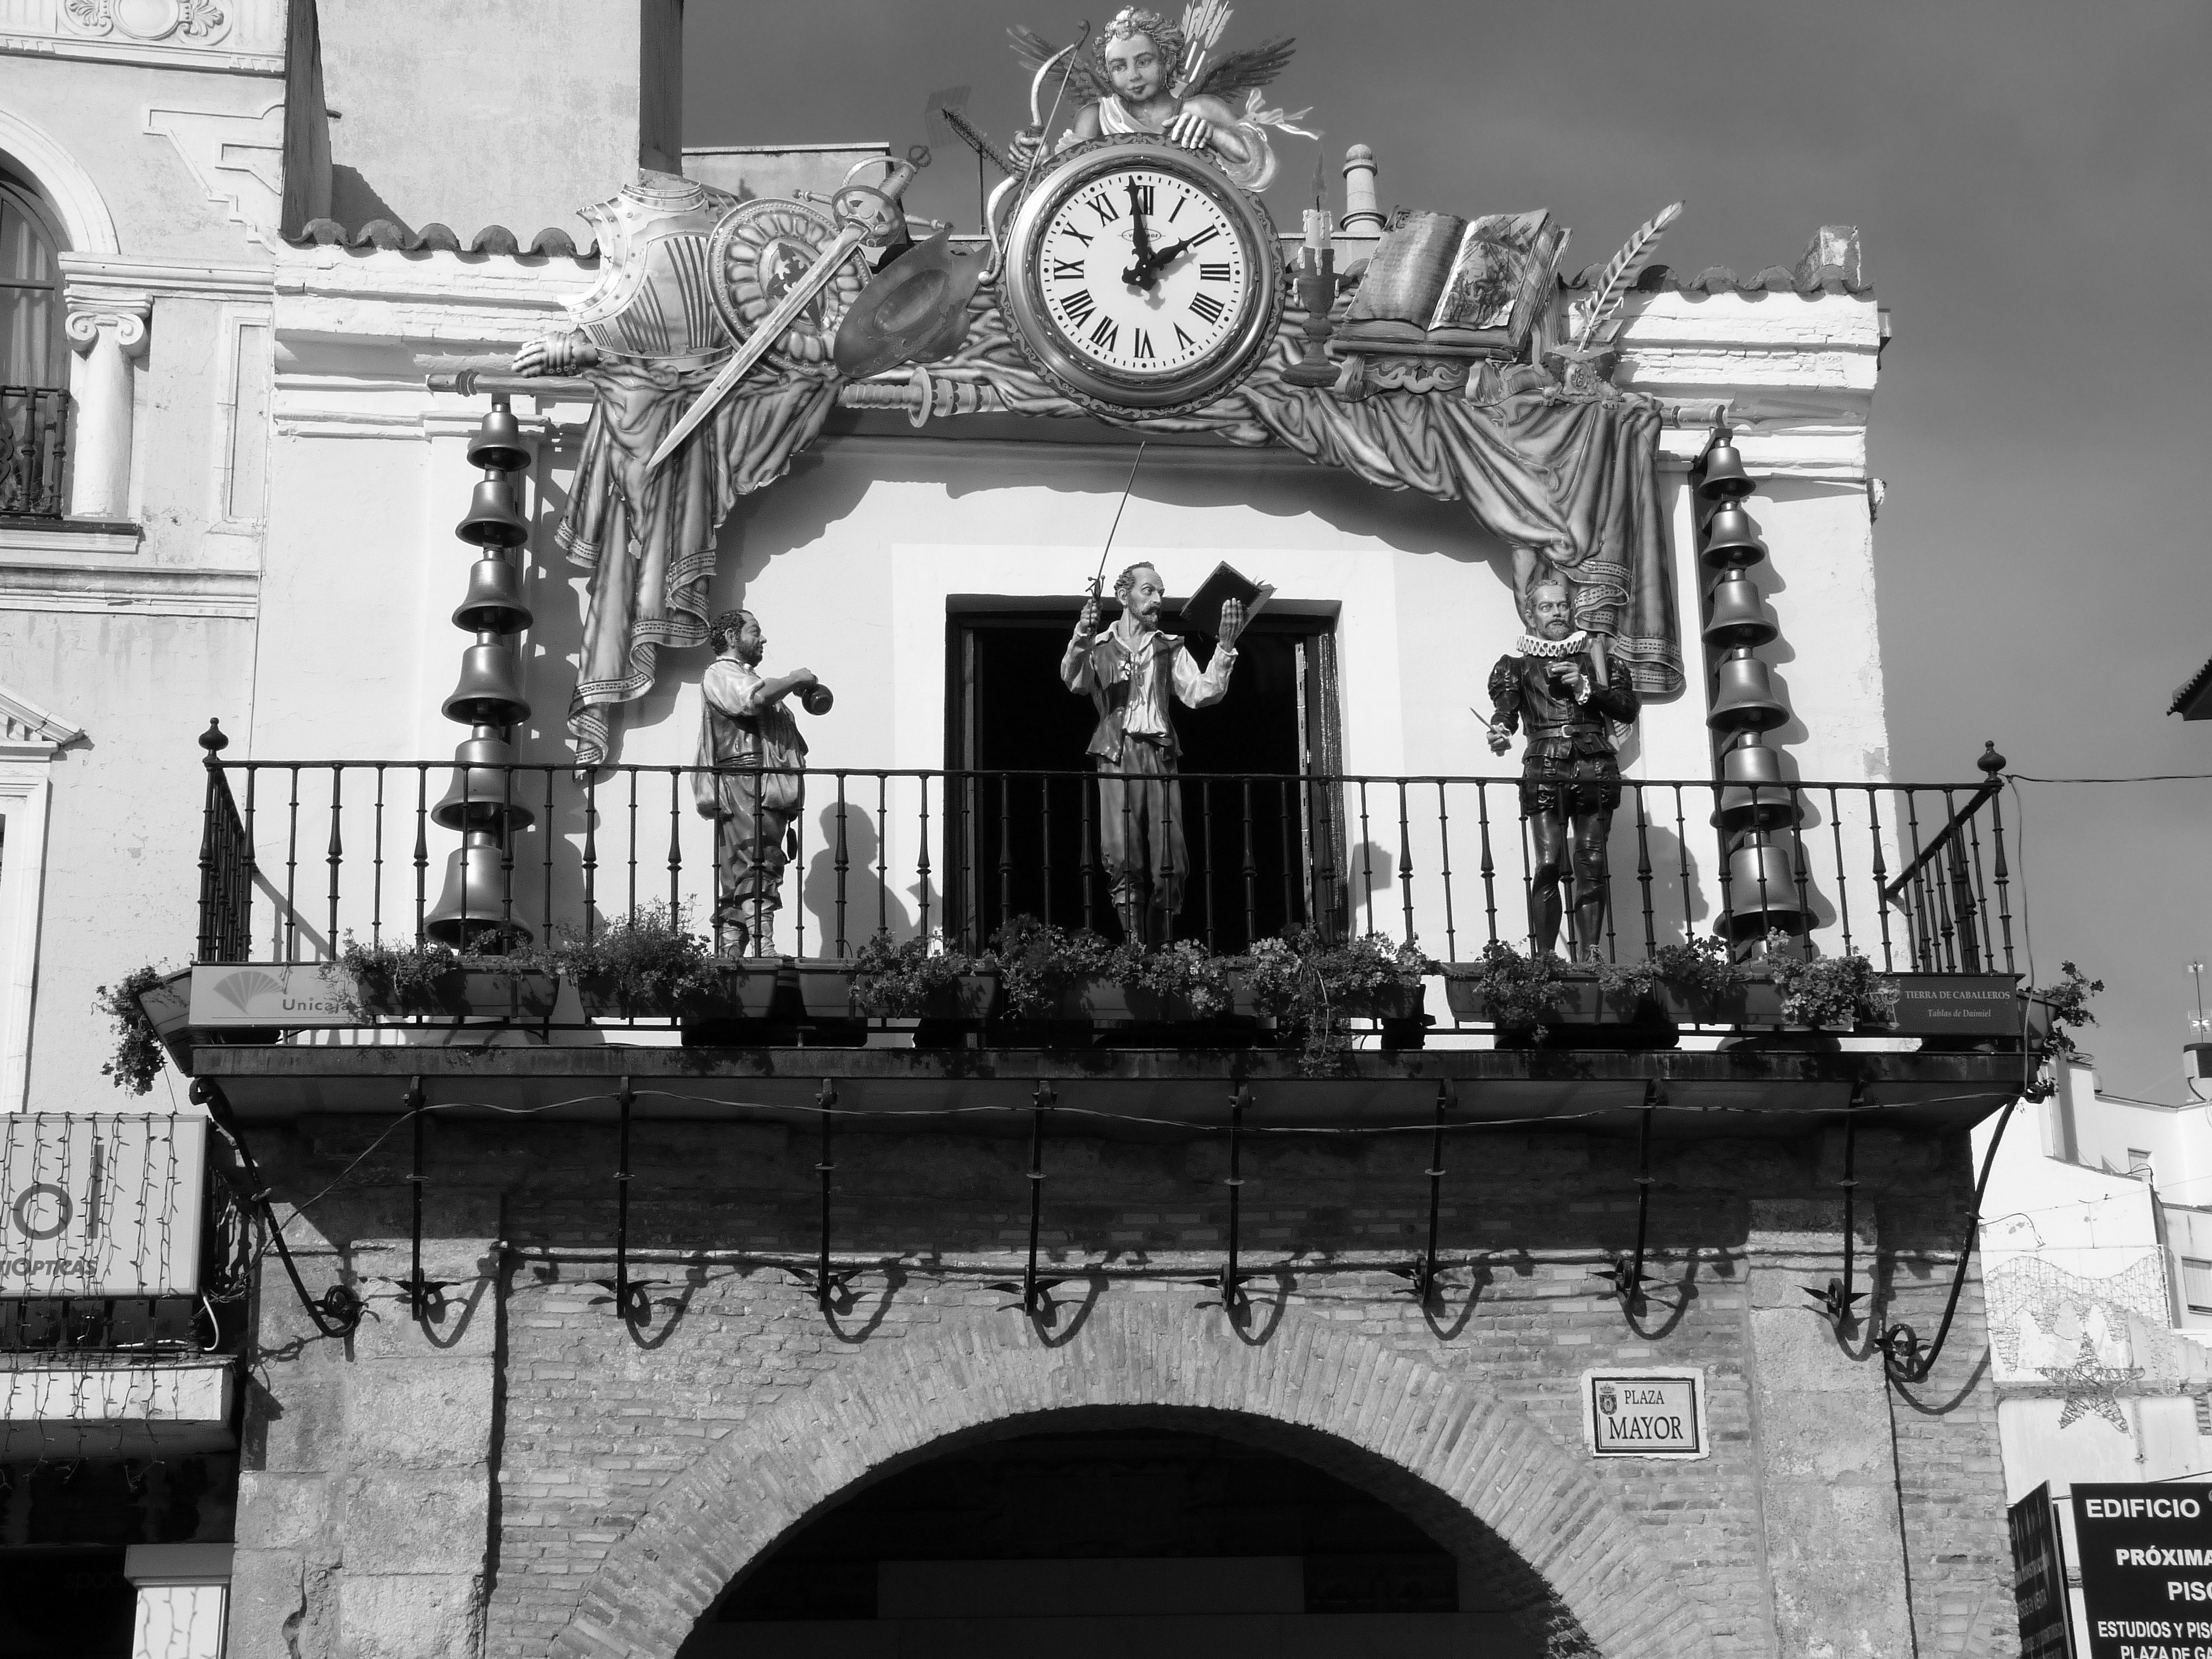
\includegraphics[width=\textwidth]{clockCRbw}
		\caption{Imagen jpg en niveles de gris}\label{fig:clockCRbw}
	\end{subfigure}
	\caption[Comparación jpg color y niveles de gris]{Ej. de paquete \texttt{subcaption} mostrando el reloj de la Plaza Mayor (cortesía de J.~Salido).}
	\label{fig:clock}
\end{figure}

\begin{figure}[hbt]
	\centering
		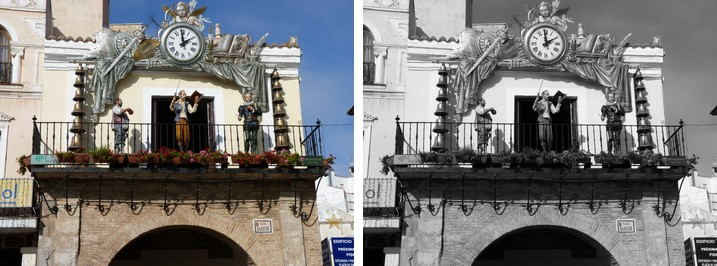
\includegraphics[width=0.97\textwidth]{2clockCR}
		\caption[Varias imágenes como una]{El reloj de la Plaza Mayor en color (izda.) y niveles de gris (dcha.).}
	\label{fig:2clock}
\end{figure}

Siempre que se tenga un fichero de imagen (mapa de bits) con un fondo blanco u otro color plano, debería intentarse transformar en una imagen con fondo transparente convirtiéndola al formato \texttt{.png} (véase ejemplo en la Fig.~\ref{fig:lion}).

\begin{figure}[hbt]
	\centering
  	\begin{subfigure}[b]{0.4\textwidth}
  		\centering
		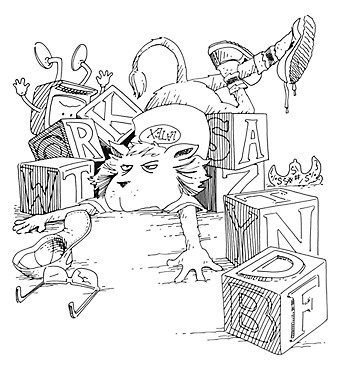
\includegraphics[width=6cm]{lionL.jpg}
		\caption{Imagen como jpg}\label{fig:lionLjpg}
  	\end{subfigure}
  	\begin{subfigure}[b]{0.4\textwidth}
  		\centering
		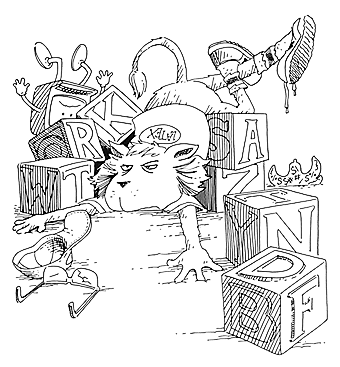
\includegraphics[width=6cm]{lionL.png}
		\caption{Imagen como png con fondo transparente}\label{fig:lionpng}
  	\end{subfigure}
  	\caption[Comparación jpg y png con transparencia]{Comparativa de formatos bitmap (cortesía de D.~Wright).}
	\label{fig:lion}
\end{figure}

Si se desea, es posible usar imágenes en color. Esto es muy conveniente para documentos electrónicos que se van a visualizar en la pantalla de un computador. Sin embargo, para documentos que serán impresos hay que tener presente si la impresión se realizará a color o en niveles de gris. 

En la Fig.~\ref{fig:escudo} se comparan los resultados obtenidos cuando la figura se inserta en formato vectorial (escalable) y cuando se hace como mapa de bits (no escalable). En este ejemplo se muestran dos versiones para el escudo de la Ingeniería Informática (cortesía de CRySoL).\footnote{El escudo basado en el núcleo de ferrita que acompaña la distribución de este documento ha sido realizado por Francisco Moya, David Villa e Ignacio Díez y su inclusión en el documento final debe respetar los derechos de la licencia CC BY-SA 3.0 con la que se distribuye.}

\begin{figure}[hbt]
	\centering
	\begin{subfigure}[b]{0.4\textwidth}
		\centering
		
\includegraphics[width=0.9\textwidth]{escudoInfBW.pdf}
		\caption{Gráfico vectorial \textsf{PDF}}\label{fig:escudoPDF}
	\end{subfigure}
	\begin{subfigure}[b]{0.4\textwidth}
		\centering
		
\includegraphics[width=0.9\textwidth]{escudoInfBW.png}
		\caption{Gráfico png}\label{fig:escudoPNG}
	\end{subfigure}
	\caption[Comparación \textsf{PDF} y png]{Comparando distintos formatos para el escudo de Informática (cortesía de CRySoL).}
	\label{fig:escudo}
\end{figure}



\subsection{Imágenes a las que se añaden gráficos}
En ocasiones es necesario recurrir a capturas de pantalla sobre las que es preciso realizar alguna anotación gráfica, por ejemplo añadiendo flechas y bloques de texto. Este es un caso que puede aparecer cuando se explica el funcionamiento de un programa informático (p.~ej.\ un manual). La captura siempre se debe llevar a cabo al mayor tamaño posible sobre la pantalla y se debe salvar en formato \texttt{.png}. Generalmente, las herramientas de captura permiten la edición de la captura añadiéndole elementos gráficos e incluso texto. En este caso los elementos añadidos 
forman parte del fichero \texttt{.png} y, por tanto, son definidos como mapa de bits. Si se desea mantener las características escalables de los elementos gráficos, éstos deben ser añadidos mediante algún programa de edición vectorial (p.~ej.\ 
\textsf{Inkscape}, \textsf{Dia}, \textsf{Visio}, etc.) y salvar el fichero resultante en formato \texttt{.pdf}. Las figs.~\ref{fig:texmk02} y \ref{fig:texmk03} muestran las diferencias en los dos procesos mencionados.

\begin{figure}[hbt]
	\centering
	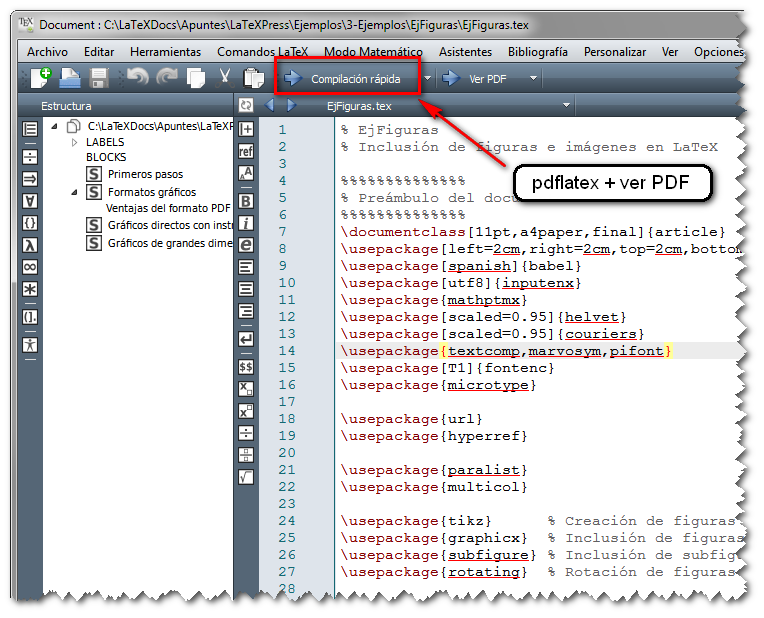
\includegraphics[width=0.6\textwidth]{texmk02} 
	\caption[Captura con gráfico en \texttt{png}]{Captura de pantalla con añadido gráfico en formato \texttt{png}.}
	\label{fig:texmk02}
\end{figure}

\begin{figure}[hbt]
	\centering
	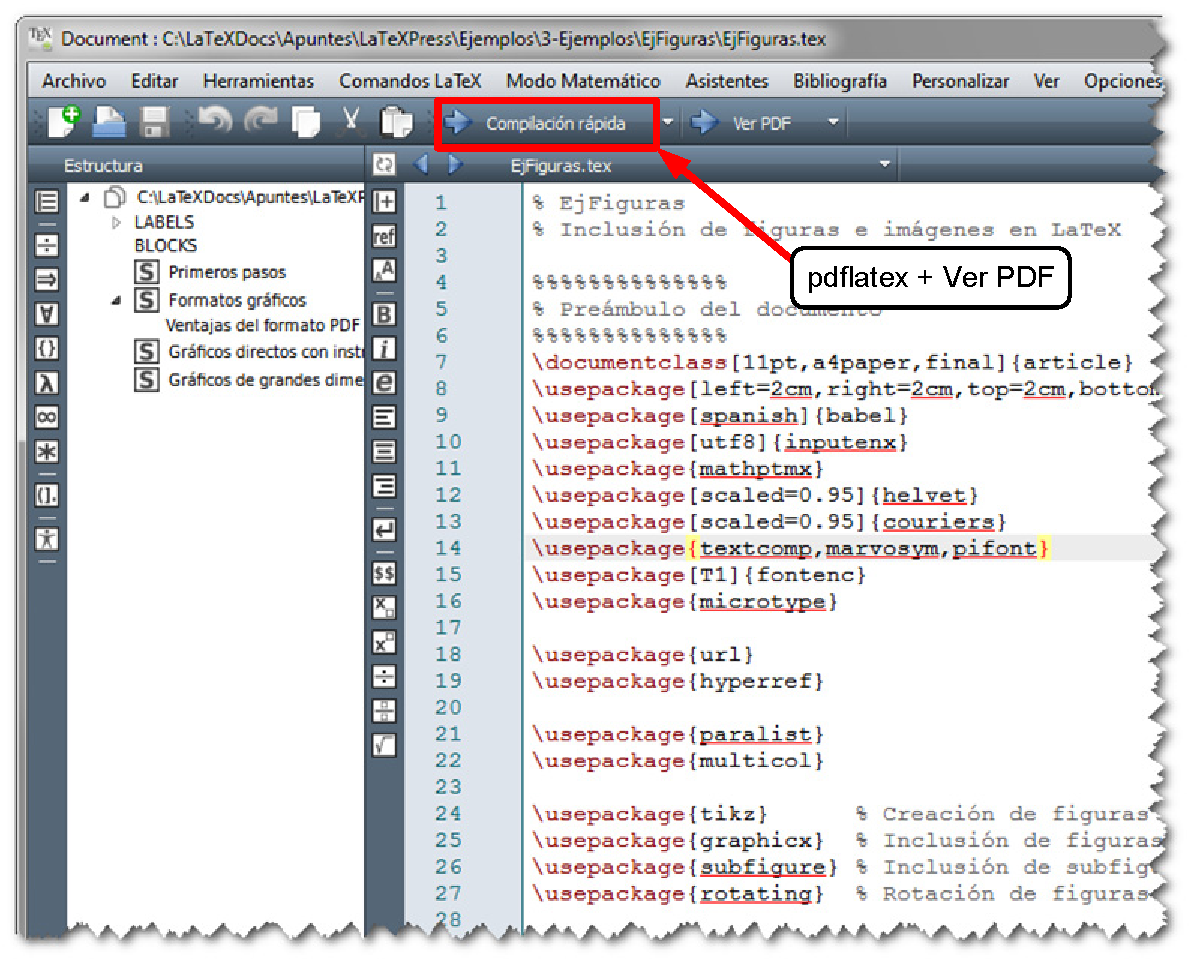
\includegraphics[width=0.6\textwidth]{texmk03} 
	\caption[Captura con gráfico en \texttt{pdf}]{Captura de pantalla con añadido gráfico en formato \texttt{pdf}.}
	\label{fig:texmk03}
\end{figure}



\subsection{Inclusión de páginas individuales de un \textsf{PDF} multipágina}
La Fig.~\ref{fig:visio_mp} nos muestra el procedimiento para usar los ficheros \textsf{PDF} multipágina\index{pdf multipágina} para incluir el gráfico de una página concreta.

\begin{figure}[hbt]
	\centering
	\includegraphics[page=2,width=0.5\textwidth]{visio_mp} 
	\caption[Gráfico de Visio multipágina]{Figura vectorial generada con Microsoft Visio en un fichero multipágina.}
	\label{fig:visio_mp}
\end{figure}



\subsection{Gráficos directos con instrucciones \TeX}
Además de los aspectos comentados aquí sobre la inclusión de imágenes y gráficos, \LaTeX{} dispone de una infinidad de recursos que pueden por sí mismo ser objeto de un curso. Un paquete muy poderoso en la generación de gráficos dentro de entornos \LaTeX{} es \texttt{tikz}\index{TikZ} (ver Fig.~\ref{fig:tikz}). La cantidad y variedad de gráficos que puede realizar es muy numerosa\footnote{Muchos ejemplos de uso en \url{http://www.texample.net/tikz/examples/}, y en especial los apartados dedicados a \href{http://www.texample.net/tikz/examples/area/electrical-engineering/}{ingeniería eléctrica} e \href{http://www.texample.net/tikz/examples/area/computer-science/}{informática}, junto con la página de web \href{https://www.kleemans.ch/diagrams-for-logic-in-latex}{<<Diagrams for Logic in \LaTeX>>}} aunque su uso requiere un conocimiento muy profundo y no es recomendable para principiantes.

\begin{figure}[hbt]
	\centering
	{\shorthandoff{>}
        \begin{tikzpicture}[scale=0.2]
        \tikzstyle{every node}+=[inner sep=0pt]
        \draw [black] (9.6,-8.7) circle (3);
        \draw (9.6,-8.7) node {$Q_0/0$};
        \draw [black] (9.6,-8.7) circle (2.4);
        \draw [black] (35,-7.9) circle (3);
        \draw (35,-7.9) node {$Q_1/1$};
        \draw [black] (35,-25.6) circle (3);
        \draw (35,-25.6) node {$Q_3/1$};
        \draw [black] (9.6,-25.6) circle (3);
        \draw (9.6,-25.6) node {$Q_2/0$};
        \draw [black] (9.6,-3.5) -- (9.6,-5.7);
        \draw (9.6,-3) node [above] {$INIT/CLR$};
        \fill [black] (9.6,-5.7) -- (10.1,-4.9) -- (9.1,-4.9);
        \draw [black] (6.782,-9.696) arc (317.19637:29.19637:2.25);
        \draw (2.23,-7.78) node [left] {$00$};
        \fill [black] (7.1,-7.07) -- (6.85,-6.16) -- (6.17,-6.89);
        \draw [black] (11.787,-6.652) arc (128.24239:55.3656:17.604);
        \fill [black] (32.69,-5.99) -- (32.31,-5.13) -- (31.75,-5.95);
        \draw (22.1,-2.34) node [above] {$01$};
        \draw [black] (35.376,-4.935) arc (200.49955:-87.50045:2.25);
        \draw (40.23,-1.77) node [above] {$10$};
        \fill [black] (37.58,-6.4) -- (38.51,-6.58) -- (38.16,-5.65);
        \draw [black] (37.962,-7.506) arc (125.31508:-162.68492:2.25);
        \draw (42.16,-10.78) node [right] {$01$};
        \fill [black] (37.11,-10.01) -- (37.17,-10.95) -- (37.99,-10.38);
        \draw [black] (12.482,-7.87) arc (104.17982:79.42817:45.722);
        \fill [black] (32.07,-7.25) -- (31.38,-6.61) -- (31.19,-7.6);
        \draw (22.21,-5.95) node [above] {$10$};
        \draw [black] (32.154,-8.847) arc (-73.76473:-102.62728:39.452);
        \fill [black] (12.5,-9.47) -- (13.17,-10.13) -- (13.39,-9.15);
        \draw (22.4,-10.95) node [below] {$00$};
        \draw [black] (37.808,-24.577) arc (137.74177:-150.25823:2.25);
        \draw (42.36,-26.44) node [right] {$11$};
        \fill [black] (37.52,-27.21) -- (37.78,-28.11) -- (38.45,-27.37);
        \draw [black] (35.751,-10.803) arc (11.59172:-11.59172:29.595);
        \fill [black] (35.75,-10.8) -- (35.42,-11.69) -- (36.4,-11.49);
        \draw (36.85,-16.75) node [right] {$00$};
        \draw [black] (8.855,-22.695) arc (-168.66522:-191.33478:28.215);
        \fill [black] (8.86,-22.7) -- (9.19,-21.81) -- (8.21,-22.01);
        \draw (7.8,-17.15) node [left] {$11$};
        \draw [black] (6.92,-26.923) arc (324:36:2.25);
        \draw (2.35,-25.6) node [left] {$10$};
        \fill [black] (6.92,-24.28) -- (6.57,-23.4) -- (5.98,-24.21);
        \draw [black] (10.124,-28.542) arc (37.82895:-250.17105:2.25);
        \draw (6.5,-32.66) node [below] {$01$};
        \fill [black] (7.58,-27.81) -- (6.64,-27.9) -- (7.26,-28.69);
        \draw [black] (11.64,-23.401) arc (135.83658:113.90487:65.965);
        \fill [black] (32.23,-9.05) -- (31.3,-8.92) -- (31.7,-9.83);
        \draw (19.74,-14.74) node [above] {$00$};
        \draw [black] (33.038,-10.169) arc (-42.35986:-67.89868:56.882);
        \fill [black] (12.41,-24.55) -- (13.34,-24.71) -- (12.96,-23.78);
        \draw (24.99,-19.01) node [below] {$11$};
        \draw [black] (12.535,-24.98) arc (100.34158:79.65842:54.397);
        \fill [black] (32.07,-24.98) -- (31.37,-24.34) -- (31.19,-25.33);
        \draw (22.3,-23.6) node [above] {$11$};
        \draw [black] (32.093,-26.339) arc (-77.62637:-102.37363:45.7);
        \fill [black] (12.51,-26.34) -- (13.18,-27) -- (13.4,-26.02);
        \draw (22.3,-27.9) node [below] {$10$};
        \draw [black] (32.845,-27.681) arc (-51.12017:-128.87983:16.799);
        \fill [black] (11.76,-27.68) -- (12.06,-28.57) -- (12.69,-27.79);
        \draw (22.3,-31.9) node [below] {$01$};
        \end{tikzpicture}
	}
	\caption[Ejemplo de gráfico con Ti\textit{K}Z]{Figura realizada con paquete \texttt{tikz} para un diagrama de transición de estados correspondiente a un autómata de Moore.}\label{fig:tikz}
\end{figure}







\subsection{Gráficos de grandes dimensiones}
Cuando se presenta la necesidad de incluir un gráfico demasiado grande para el tamaño de la página una opción muy apropiada es la impresión del gráfico en modo apaisado en una página aparte. Este efecto se consigue con el entorno \texttt{sidewaysfigure}\index{sidewaysfigure} proporcionado por el paquete \texttt{rotating}.\index{rotating} La Fig.~\ref{fig:sideways} muestra un ejemplo del entorno citado con un gráfico \textsf{PDF}.

\begin{sidewaysfigure}
	\centering
	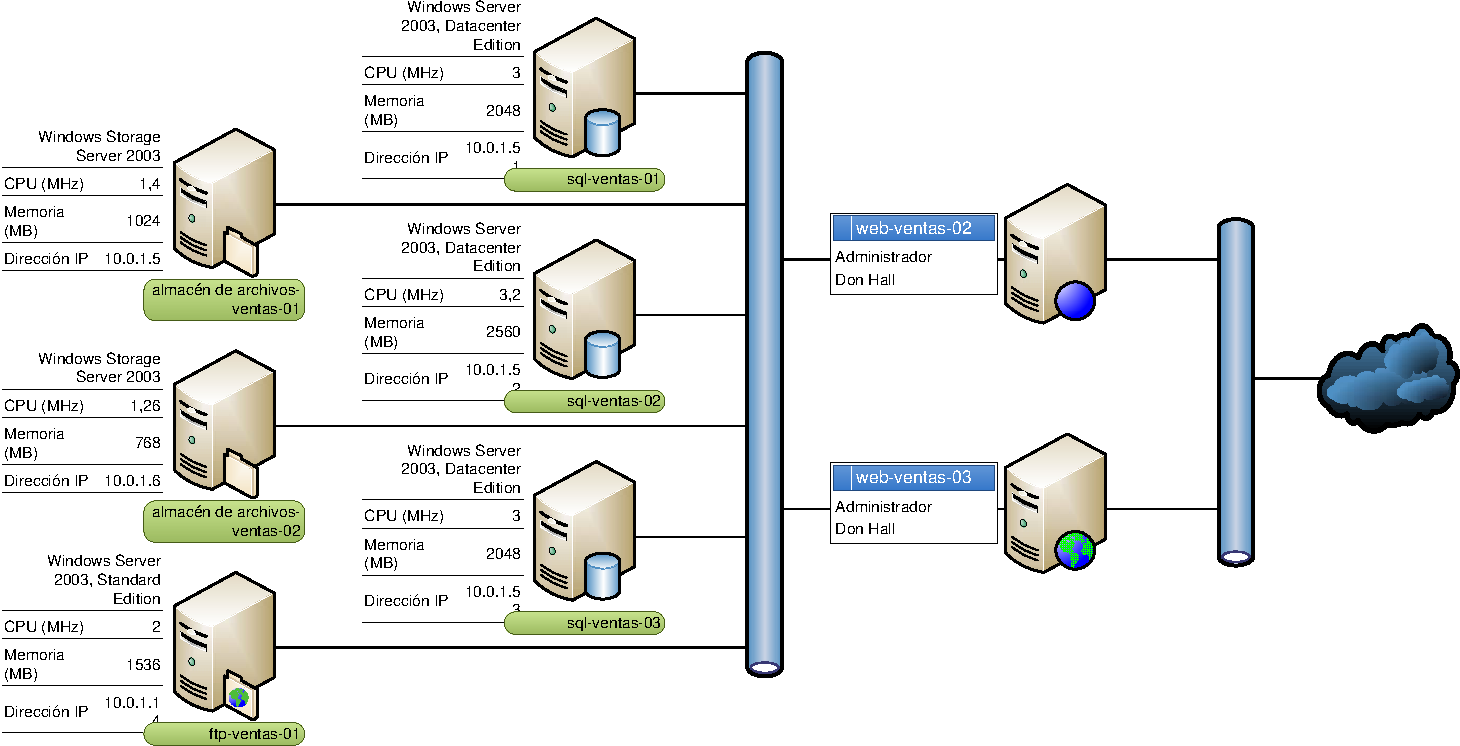
\includegraphics[width=0.98\textheight]{network} 
	\caption[Gráfico de apaisado Visio]{Figura vectorial con impresión apaisada.}
	\label{fig:sideways}
\end{sidewaysfigure}






\chapter{Tablas en \LaTeX{}}
La inclusión de tablas en documentos preparados con \LaTeX{} no es sencilla e incluso podría calificarse de <<engorrosa>>. Las tablas se crean con el entorno \texttt{tabular} en el que se indica el número de columnas y la alineación del texto en cada columna (l=izda., c=central, r=dcha.). Las líneas de separación en la tabla se indican mediante el carácter \texttt{`|'} (líneas verticales) o la macro \texttt{\textbackslash hline} (líneas horizontales). La separación del texto entre columnas se realiza con el carácter \texttt{`\&'} y la separación de filas con \texttt{`\textbackslash\textbackslash'}.

Para que la tabla sea manejada como un objeto \emph{float} debe incluirse en el entorno \texttt{table}, cuya ubicación se rige por los mismos principios que la inclusión de figuras o cualquier otro objeto flotante.

Un sitio muy apropiado para experimentar con las tablas y aprender los principios básicos de eso se proporciona en: \url{www.learnlatex.org/es/lesson-08}. En este sitio puedes encontrar una explicación sucinta de la creación de tablas en \LaTeX{} con numerosos ejemplos con los que practicar y que reproducimos en este documento.

Para obtener una interfaz mejorada de creación de entornos tabular en \LaTeX{} siempre se debe cargar el paquete \texttt{array}.\index{array} En el ejemplo de la tabla~\ref{tab:simple} se muestra una tabla con un conjunto importante de propiedades como: líneas de separación (horizontales y verticales), distintos tipos de justificación, etc. Como puede comprobarse en dicho ejemplo, \LaTeX{} es capaz de realizar las tablas con multitud de elementos con una gran flexibilidad. Sin embargo, echando un vistazo al texto fuente podemos intuir que la elaboración de tablas es tediosa y tanto más cuanto mayor sea el tamaño y la complejidad de la tabla. Por supuesto, las tablas creadas en \LaTeX{} son armoniosas y congruentes con el texto general. Por ello, la inmensa mayoría de publicaciones científicas exigen que las tablas sean creadas de modo nativo mediante comandos \LaTeX{} y no se permite su inclusión como figura (p.~ej., de una captura de pantalla).

\begin{table}[H]%
	\centering
	\caption[Ejemplo de entorno \texttt{table}]{Tabla sencilla}		  \label{tab:simple}
    \begin{tabular}{l|l|l}
      \textbf{Animal}  & \textbf{Comida} & \textbf{Tamaño} \\
      \hline
      perro   & carne  & mediano \\
      caballo & heno   & grande  \\
      rana    & moscas & pequeño \\
    \end{tabular}
\end{table}

En el siguiente ejemplo se ha hecho uso de la macro \texttt{cline}\index{cline} para generar líneas que no abarcan todas las columnas de la tabla.

\begin{table}[H]%
	\centering
	\caption{Ejemplo de uso de la macro \texttt{cline}}
	\label{tab:cline}
	\begin{tabular}[t]{|r|l|}
	\hline
	7C0 & hexadecimal \\[1cm] % Ejemplo de separación fijada entre líneas
	3700 & octal \\ \cline{2-2}
	11111000000 & binario \\
	\hline \hline
	1984 & decimal \\
	\hline
	\end{tabular}
\end{table}

Hay que tener cuidado con la longitud del contenido de cada celda, ya que por defecto, \LaTeX{} no recorta el texto al tamaño de la línea. Para evitarlo se especifica el ancho de columna:

\begin{table}[H]%
	\centering
	\caption{Ejemplo de tabla con especificación de anchura de columna}
	\label{tab:anchura}
	\begin{tabular}{ | l | l | l | p{5cm} |}
	\hline
	Día & Temp Mín (\textdegree C) & Temp Máx (\textdegree C) & Previsión \\ \hline
	Lunes & 11 & 22 & Día claro y muy soleado. Sin embargo, la brisa de la tarde puede hacer que las temperaturas desciendan \\ \hline
	Martes & 9 & 19 & Nuboso con chubascos en muchas regiones. En Cataluña claro con posibilidad de bancos nubosos al norte de la región \\ 
    \hline
	\end{tabular}
\end{table}

Cuando las tablas tienen muchas columnas es posible hacer una declaración abreviada empleando la sintaxis \texttt{*\{num\}\{just\}} como en la tabla siguiente:

\begin{table}[H]%
	\centering
	\caption{Especificación abreviada en tabla}
	\label{tab:abreviada}
	\begin{tabular}{l*{6}{c}|r}
	Equipo            & J & G & P & E & F  & C & Pts \\
	\hline
	Manchester United & 6 & 4 & 0 & 2 & 10 & 5 & 12  \\
	Celtic            & 6 & 3 & 0 & 3 &  8 & 9 &  9  \\
	Benfica           & 6 & 2 & 1 & 3 &  7 & 8 &  7  \\
	FC Copenhagen     & 6 & 2 & 1 & 2 &  5 & 8 &  7  \\
	\end{tabular}
\end{table}









\section{Tablas profesionales}
Un pequeño consejo antes de introducir las líneas; en las tablas las líneas deben ser usadas con mesura y normalmente las líneas verticales no parecen ser de un uso muy profesional. De hecho, para las tablas profesionales no debe utilizar ninguna de las líneas estándar; en su lugar usted debe familiarizarse con las que le facilita el paquete \texttt{booktabs}.\index{booktabs} Este paquete proporciona cuatro tipos diferentes de líneas. Cada uno de los comandos que permiten definirlas, deben ser el primer elemento de una fila o seguir a otra línea ya definida. Tres de estos comandos son: \textbackslash \texttt{toprule}, \textbackslash \texttt{midrule} y \textbackslash \texttt{bottomrule} que son usados para situar una línea en la parte alta, en las filas intermedias o en la parte baja de la tabla, respectivamente, 

El cuarto comando proporcionado por \texttt{booktabs} es \textbackslash \texttt{cmidrule}. Puede ser usado para dibujar una línea que no se extienda a toda la fila de una tabla, sino a un intervalo específico de columnas de esa fila. Debe especificarse un intervalo de columnas de la forma: \texttt{\{n-n\}}. Incluso si se desea dibujar una línea para una única columna, se debe especificar como un intervalo (siendo los extremos del intervalo el mismo número).

\begin{table}[H]
   \centering
   	  \caption{Tabla con paquete \texttt{booktabs}}
   	  \label{tab:booktabs}      
   	  \begin{tabular}{llr}
      \toprule
      \multicolumn{2}{c}{Item} \\
      \cmidrule(r){1-2}
      Animal & Description & Price (\$) \\
      \midrule
      Gnat  & per gram & 13.65 \\
            & each     &  0.01 \\
      Armadillo & frozen & 8.99 \\
      \bottomrule
      \end{tabular}
\end{table}

Existe otro uso útil de \texttt{\textbackslash cmidrule}. Puede acortar el principio o fin de una línea o incluso con un argumento opcional entre paréntesis, donde \texttt{r} y \texttt{l} significan que la línea se acorta a la derecha (right) o a la izquierda (left), respectivamente.

\begin{table}[H]
   \centering
   	  \caption{Tabla con varios tipos de líneas.}
   	  \label{tab:cmidrule}      
    \begin{tabular}{lll}
      \toprule
      Animal  & Comida & Tamaño  \\
      \midrule
      perro   & carne  & mediano \\
      \cmidrule{1-2}
      caballo & heno   & grande  \\
      \cmidrule(r){1-1}
      \cmidrule(rl){2-2}
      \cmidrule(l){3-3}
      rana    & moscas & pequeño \\
      \bottomrule
    \end{tabular}
\end{table}

Algunas veces una línea puede implicar una fuerte separación, no deseada, entre dos filas, pero en aras de una mayor claridad es posible que se desee separar esas líneas de alguna manera. En este caso se puede usar \texttt{\textbackslash addlinespace}\index{addlinespace} que añadirá un pequeño espacio vertical entre ambas.

\begin{table}[H]
   \centering
   	  \caption{Tabla con espacio extra entre filas.}
   	  \label{tab:espace}      
    \begin{tabular}{cp{9cm}}
      \toprule
      Animal & Descripción \\
      \midrule
      perro  & El perro es un miembro del género Canis, el cual forma parte 
               de los cánidos derivados del lobo. \\
      \addlinespace
      gato   & El gato es una especie doméstica de pequeños mamíferos carnívoros. Es la 
               única especie domesticada de la familia de los félidos y es a menudo llamado 
    		   gato doméstico. \\
      \bottomrule
    \end{tabular}
\end{table}






\section{Expansión de celdas a filas y columnas}
El paquete \texttt{multirow}\index{multirow} permite la expansión de celdas a varias columnas o filas empleando los comandos \texttt{multicolum}\index{multicolum} y \texttt{multirow} como se muestra en los siguientes ejemplos:

\begin{table}[H]%
	\centering
	\caption{Ejemplo de expansión en columnas}
	\label{tab:expcolumnas}
	\begin{tabular}{|l|l|} % Expansión en columnas
	\hline
	\multicolumn{2}{|c|}{Alineación} \\
	\hline
	GK & Paul Robinson \\
	LB & Lucus Radebe \\
	FW & Jamie McMaster \\
	ST & Alan Smith \\
	ST & Mark Viduka \\
	\hline
	\end{tabular}
\end{table}

\begin{table}[H]%
	\centering
	\caption{Ejemplo de expansión en filas}
	\label{tab:expfilas}
	\begin{tabular}{|l|l|l|} % Expansión en filas
	\hline
	\multicolumn{3}{|c|}{Alineación} \\
	\hline
	Guardameta & GK & Paul Robinson \\ \hline
	\multirow{4}{*}{Defensas} & LB & Lucus Radebe \\
	 & DC & Michael Duberry \\
	 & DC & Dominic Matteo \\
	 & RB & Didier Domi \\ \hline
	\multirow{3}{*}{Centrocampistas} & MC & David Batty \\
	 & MC & Eirik Bakke \\
	 & MC & Jody Morris \\ \hline
	Delanteros & FW & Jamie McMaster \\ \hline
	\multirow{2}{*}{Puntas} & ST & Alan Smith \\
	 & ST & Mark Viduka \\
	\hline
	\end{tabular}
\end{table}



\begin{table}[H]%
	\centering
	\caption{Ejemplo de expansión simultánea en filas y columnas}
	\label{tab:expsimul}
	\begin{tabular}{cc|c|c|c|c|l} % Expansión simultánea en filas y columnas
	\cline{3-6}
	& & \multicolumn{4}{|c|}{Primos} \\ \cline{3-6}
	& & 2 & 3 & 5 & 7 \\ \cline{1-6}
	\multicolumn{1}{|c|}{\multirow{2}{*}{Potencias}} &
	\multicolumn{1}{|c|}{504} & 3 & 2 & 0 & 1 &     \\ \cline{2-6}
	\multicolumn{1}{|c|}{}                        &
	\multicolumn{1}{|c|}{540} & 2 & 3 & 1 & 0 &     \\ \cline{1-6}
	\multicolumn{1}{|c|}{\multirow{2}{*}{Potencias}} &
	\multicolumn{1}{|c|}{mcd} & 2 & 2 & 0 & 0 & min \\ \cline{2-6}
	\multicolumn{1}{|c|}{}                        &
	\multicolumn{1}{|c|}{mcm} & 3 & 3 & 1 & 1 & max \\ \cline{1-6}
	\end{tabular}
\end{table}








\section{Alienación de columnas con información numérica}
Cuando se emplean tablas con datos numéricos a veces puede interesar la alineación de datos por el signo de puntuación empleado para la separación de decimales (\texttt{`,'} en español, \texttt{`.'} en inglés). Un ejemplo de esto se ilustra a continuación:

\begin{table}[H]%
	\centering
	\caption{Tabla numérica con alineación al carácter `,'}
	\label{tab:alineada}
	\begin{tabular}{c r@{,} l}
    \toprule
	Expresión con pi & \multicolumn{2}{c}{Valor} \\
	\midrule
	$\pi$                   &      3 & 14159 \\
	$\pi^{\pi}$             & 36     &    46 \\
	$(\pi^{\pi})^{\pi}$     &  80662 & 7     \\
    \bottomrule
	\end{tabular}
\end{table}

Cuando se trata de trabajar con números y unidades físicas, existen paquetes especializados en su tratamiento tipográfico adecuado. Quizá el más interesante es \texttt{siunitx}\index{siunitx} que se encarga de los aspectos mencionados para el idioma concreto de uso y las unidades empleadas del SI. Dicho paquete también añade un nuevo identificador de columna en las tablas cuando estas contienen información numérica (compara Tablas~\ref{tab:alineada} y \ref{tab:siunitx}).

\begin{table}[H]%
	\centering
	\caption{Tabla numérica con alineación al carácter `,' obtenido mediante paquete \texttt{siunitx}}
	\label{tab:siunitx}
	\begin{tabular}{c S}
    \toprule
	Expresión con pi & Valor \\
	\midrule
	$\pi$                   & 3,14159 \\
	$\pi^{\pi}$             & 36,46 \\
	$(\pi^{\pi})^{\pi}$     & 80662,7 \\
    \bottomrule
	\end{tabular}
\end{table}









\section{Tablas con mayor control del espaciado}
En el entorno tabular el control del espaciado entre columnas es demasiado <<burdo>>. Para facilitar esta labor existen paquetes como \texttt{tabularx}, cuyo uso se muestra en los ejemplos siguientes:\index{tabularx}

\begin{table}[H]
   \centering
   	\caption{Ejemplo de tabla con entorno\texttt{tabularx}}					\label{tab:tabularx1}
   \begin{tabularx}{\textwidth}% Se especifica el ancho completo de la tabla
   { |X|X|X|r| }
   \hline
   etiqueta 1 & etiqueta 2 & etiqueta 3 & etiqueta 4 \\
   \hline
   ítem 1     & ítem 2     & ítem 3     & ítem 4  \\
   \hline
	\end{tabularx}
\end{table}


\begin{table}[H]
	\newcolumntype{R}{>{\raggedleft\arraybackslash}X}%
	\centering
    \caption{Otro ejemplo de tabla ampliada}
    \label{tab:tabularx2}
	\begin{tabularx}{\textwidth}{ |l|R|l|R| }
  	\hline
   etiqueta 1 & etiqueta 2 & etiqueta 3 & etiqueta 4 \\
   \hline
   ítem 1     & ítem 2     & ítem 3     & ítem 4  \\
  	\hline
   \end{tabularx}
\end{table}

Otros ejemplos:

\begin{center}
\begin{tabular}{lp{2cm}}
\hline
A & B B B B B B B B B B B B B B B B B B B B B B B B\\
C & D D D D D D D\\
\hline
\end{tabular}
\end{center}

\begin{center}  
\begin{tabularx}{.5\textwidth}{lX}
\hline
A & B B B B B B B B B B B B B B B B B B B B B B B B\\
C & D D D D D D D\\
\hline
\end{tabularx}
\end{center}

\begin{center}  
\begin{tabularx}{\textwidth}{lX}
\hline
A & B B B B B B B B B B B B B B B B B B B B B B B B\\
C & D D D D D D D\\
\hline
\end{tabularx}
\end{center}





\section{Tablas con color}
El uso del color en los documentos académicos debe realizarse de modo muy comedido y sólo cuando el mismo sea fundamental para facilitar la comprensión de los contenidos expuestos. En las tablas se puede hace uso del color si se emplea el paquete \texttt{xcolor}\index{xcolor} con la opción \texttt{table}.

\begin{table}[H]
	\centering
	\caption{Tabla con filas de colores alternados}
	\rowcolors{2}{gray!10}{gray!40}
	\begin{tabular}{lll}
    \toprule
		Col. 1  & Col. 2  & \cellcolor{red!40}Col. 3 \\
    \midrule
		par    & par    & par   \\
		impar  & impar  & impar \\
		par    & par    & par   \\
		impar  & impar  & impar \\
		par    & par    & par   \\
    \bottomrule
	\end{tabular}
\end{table}

\begin{table}[H]
	\centering
	\caption{Tabla con una columna en color}
	\begin{tabular}{ll>{\columncolor{green!20}}l}
    \toprule
		Col. 1  & Col. 2  & Col. 3 \\
    \midrule
		par    & par    & par   \\
		impar  & impar  & impar \\
		par    & par    & par   \\
    \bottomrule
	\end{tabular}
\end{table}





\section{Tablas de gran tamaño}
Puede ocurrir que debido al tamaño de la tabla, quede mejor girada en la página para obtener una orientación apaisada. Este efecto se puede conseguir de un modo sencillo con el paquete \texttt{rotating} que no es preciso cargar explícitamente si se emplea el paquete \texttt{graphicx}. Para conseguir el efecto mencionado se empleará el entorno \texttt{sidewaystable},\index{sidewaystable} como se muestra en el caso de la tabla~\ref{tab:apaisada}.

El paquete \texttt{graphicx} aporta comandos para realizar el escalado de objetos en un documento \LaTeX. Un caso interesante es el escalado para adaptar el tamaño de una tabla, aunque esto se debe hacer con sumo cuidado, ya que el tamaño de las fuentes empleadas en la tabla quedará afectado en el mismo factor de escala aplicado y no se corresponderá con el tamaño del texto de una tabla normal. En la tabla~\ref{tab:escalada} se muestra el efecto de escalado para ajustar su tamaño al de la página.

\begin{sidewaystable}
	\centering
	\caption[Ejemplo de tabla apaisada]{Tabla apaisada en una página}\label{tab:apaisada}
	\begin{tabular}{llllllllp{1in}lp{1in}}
		\toprule
		Context   &Length   &Breadth/   &Depth   &Profile   &Pottery   &Flint   &Animal   &Stone   &Other    &C14 Dates \\
		&         &Diameter   &        &          &          &        & 
		Bones&&&\\
		\midrule
		&&&&&&&&&&\\
		\multicolumn{10}{l}{\bf Grooved Ware}&\\
		784       &---        &0.9m       &0.18m   &Sloping U &P1       &$\times$46  &  $\times$8      &&       $\times$2 bone&  2150$\pm$ 100 BC\\
		785       &---        &1.00m      &0.12    &Sloping U &P2--4    &$\times$23  &  $\times$21     & Hammerstone &---&---\\
		962       &---        &1.37m      &0.20m   &Sloping U &P5--6    &$\times$48  &  $\times$57*    & ---&     ---&1990 $\pm$ 80 BC (Layer 4) 1870 $\pm$90 BC (Layer 1)\\
		983       &0.83m      &0.73m      &0.25m   &Stepped U &---      &$\times$18  &  $\times$8      & ---& Fired clay&---\\
		&&&&&&&&&&\\
		\multicolumn{10}{l}{\bf Beaker}&\\
		552       &---        &0.68m      &0.12m   &Saucer    &P7--14   &---           & ---       & ---       &---        &---\\
		790       &---        &0.60m      &0.25m   &U         &P15      &$\times$12    & ---       & Quartzite-lump&---    &---\\
		794       &2.89m      &0.75m      &0.25m   &Irreg.    &P16      &$\times$3     & ---       & ---       &---        &---\\
		\bottomrule
	\end{tabular}
\end{sidewaystable}


\begin{table}[H]
	\centering
	\caption{Tabla escalada}
	\label{tab:escalada}
	\resizebox{\textwidth}{!}{% En el escalado ajustamos sólo el ancho para mantener la proporción
		\begin{tabular}{llllllllp{1in}lp{1in}}
			\toprule
			Context   &Length   &Breadth/   &Depth   &Profile   &Pottery   &Flint   &Animal   &Stone   &Other    &C14 Dates \\
			&         &Diameter   &        &          &          &        & 
			Bones&&&\\
			\midrule
			&&&&&&&&&&\\
			\multicolumn{10}{l}{\bf Grooved Ware}&\\
			784       &---        &0.9m       &0.18m   &Sloping U &P1       &$\times$46  &  $\times$8      &&       $\times$2 bone&  2150$\pm$ 100 BC\\
			785       &---        &1.00m      &0.12    &Sloping U &P2--4    &$\times$23  &  $\times$21     & Hammerstone &---&---\\
			962       &---        &1.37m      &0.20m   &Sloping U &P5--6    &$\times$48  &  $\times$57*    & ---&     ---&1990 $\pm$ 80 BC (Layer 4) 1870 $\pm$90 BC (Layer 1)\\
			983       &0.83m      &0.73m      &0.25m   &Stepped U &---      &$\times$18  &  $\times$8      & ---& Fired clay&---\\
			&&&&&&&&&&\\
			\multicolumn{10}{l}{\bf Beaker}&\\
			552       &---        &0.68m      &0.12m   &Saucer    &P7--14   &---           & ---       & ---       &---        &---\\
			790       &---        &0.60m      &0.25m   &U         &P15      &$\times$12    & ---       & Quartzite-lump&---    &---\\
			794       &2.89m      &0.75m      &0.25m   &Irreg.    &P16      &$\times$3     & ---       & ---       &---        &---\\
			\bottomrule
	\end{tabular}}
\end{table}




\section{Tablas incluidas como figuras}
Tal como muestran los ejemplos precedentes la preparación de tablas con \LaTeX{} es un proceso de cierta complejidad. Por el contrario las tablas, confeccionadas mediante hojas de cálculo, que puede incluirse en los documentos con los procesadores tipo \textsc{WYSIWYG} (\textsf{Word}, \textsf{OpenOffice}, etc.) siguen un proceso intuitivo y rápido. Existe un modo para aprovechar estas ventajas empleando \LaTeX{}. Para ello se puede salvar en formato \textsf{PDF} las tablas creadas con una hoja de cálculo (p.~ej.\ \textsf{Excel}) e incorporarlas en un documento \LaTeX{} mediante una tabla que sólo contiene una celda en la que incluimos el fichero gráfico con la tabla en formato \textsf{PDF}. 

La tabla~\ref{tab:figura} muestra un ejemplo de tabla creada con \textsf{Excel} e incluida como un fichero \textsf{PDF}. Este método permite emplear las tipografías disponibles en el sistema para las hojas de cálculo. Además, se pueden aplicar todas las opciones aplicables para los gráficos incluido el dimensionado de los mismos. Es importante señalar que si no se va a aplicar ningún escalado a la figura de la tabla, ésta debería crearse con el mismo tamaño de fuente que tendrá el texto normal del documento final y empleando preferiblemente una tipografía similar a la utilizada en el documento.

\begin{table}[H]%
	\centering
	\caption[Tabla \textsf{Excel}]{Ejemplo de tabla creada con \textsf{Excel} e incluida como figura}
	\label{tab:figura}
	\begin{tabular}{c}
		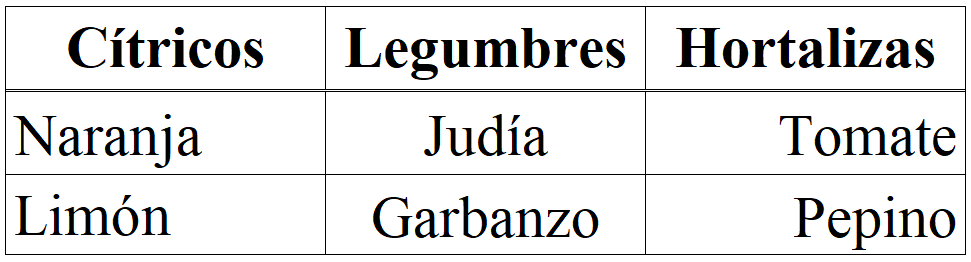
\includegraphics{alimentos}
	\end{tabular}
\end{table}

Este método es aceptable para publicaciones como TFG y Tesis. Sin embargo, no es apropiado para publicaciones especializadas (p.~ej.\ revistas y congresos) y en estos casos la editorial suele rechazar el resultado por los estándares tan exigentes empleados. El problema deriva de que las fuentes empleadas por los programas externos emplean tipografías ligeramente diferentes a las empleadas por \LaTeX.




\chapter{Fórmulas matemáticas}
Para que \LaTeX{} pueda incluir muchos símbolos matemáticos es preciso incluir algunos paquetes que ayudan en dicha tarea: \texttt{amsmath}, \texttt{amsfonts}, \texttt{amssymb}. También hay que tener en cuenta que si el tipo principal empleado en el texto es Times y se desea utilizar un tipo coherente en las fórmulas es conveniente emplear el paquete \emph{mathptmx} en vez de \emph{Times}. Pero en este caso es recomendable incluir siempre paquetes adicionales para suministrar las otras dos familias de fuentes escalables (p.~ej.\ \texttt{helvet} para familia \textsf{palo seco} y \texttt{couriers} para \texttt{monoespaciada}). Si no se hace esta última inclusión pueden obtenerse errores de difícil diagnóstico.








\section{Fórmulas creadas en línea y con entorno \texttt{equation}}
Es muy sencillo incluir fórmulas matemáticas sencillas en el mismo texto en el que se escribe. Por ejemplo, $c^{2}=a^{2}+b^{2}$ que podría ser la ecuación representativa del teorema de Pitágoras.

Las fórmulas también se pueden separar del texto para que aparezcan destacadas, así:

% Ejemplo: Ecuación no numerada
% ============
\[
c^2  = \int {\left( {a^2  + b^2} \right)}  \cdot dx
\]


Pero si se desea, las ecuaciones pueden ser numeradas de forma automática e incluso utilizar referencias cruzadas a ellas:

% Ejemplo: Ec. numerada.
% ============
\begin{equation} \label{eq:pitagoras}
	a^{2}=b^{2} + \cancel{c^{2}}+ \xcancel{d^{2}}
\end{equation}

Como vemos en la ecuación~\ref{eq:pitagoras} algunos términos podemos señalarlos como cancelados, gracias al paquete \texttt{cancel}.\footnote{\url{https://osl.ugr.es/CTAN/macros/latex/contrib/cancel/cancel.pdf}} Otras formas de \sout{subrayar} el texto se consiguen con el paquete \uwave{\texttt{ulem}}.\footnote{\url{https://osl.ugr.es/CTAN/macros/latex/contrib/ulem/ulem.pdf}}

\bigskip
Las macros que proporciona el paquete \texttt{ulem} son:
\begin{itemize}[noitemsep]
	\item \verb|\uline{importante}|: texto subrayado como \uline{importante}.
	
	\item \verb|\uuline{urgente}|: doble subrayado como \uuline{urgente}.
	
	\item \verb|\uwave{ondulado}|: subrayado \uwave{ondulado}.
	 
	\item \verb|\sout{tachado}|: texto \sout{tachado}.
	
	\item \verb|\xout{cruzado}|: texto \xout{cruzado}.
	
	\item \verb|\dashuline{discontinuo}|: subrayado \dashuline{discontinuo}.
	 
	\item \verb|\dotuline{punteado}|: subrayado \dotuline{punteado}.
\end{itemize}
\bigskip

No hay que preocuparse demasiado por la tipografía empleada en las fórmulas pues \LaTeX{} hace por nosotros <<casi>> todo el trabajo.\footnote{Los matemáticos son muy exquisitos y no se conforman con cualquier cosa, pero nosotros debemos ser mucho menos pretenciosos si queremos resultados rápidos.}

Los ejemplos que aquí se muestran son muy sencillos pero \LaTeX{} proporciona entornos específicos más potentes. Para mostrar algo <<más sofisticado>> añado dos ejemplos más. La ec.~\ref{eq:integral} que es un poquito más compleja y la ec.~\ref{eq:cuadro} que está recuadrada.

% Ejemplo:
% ============
\begin{equation}\label{eq:integral}
	I = \! \int_{-\infty}^\infty f(x)\,dx
\end{equation}

Un ejemplo de alineación de ecuación mediante entorno \texttt{flalign}:\footnote{Otra forma de conseguir el alineamiento a la izquierda de las ecuaciones se consigue añadiendo \texttt{fleqn} como opción de la clase del documento.}
\begin{flalign}
    &f(x) = -1.25x^{2} + 1.5x&
\end{flalign}

En este caso la versión con estrella (\texttt{flalign*}) suprime la numeración de la ecuación.

% Ejemplo: Ec. con recuadro (numeración exterior).
% ============
{\fboxsep 8pt \fboxrule 2.5pt 
%\fboxsep ajusta la separación entre la caja y el elemento recuadrado
%\fboxrule ajusta el espesor de la línea del recuadro
\begin{equation}\label{eq:cuadro}
\fbox{$\displaystyle 
R = \frac{L}{2} \cdot \frac{{\left( {v_d  + v_i } \right)}}{{\left( {v_d  - v_i } \right)}}
$}
\end{equation}
}


Algunos otros cuadros en ecuaciones son p.~ej.\ $x + y = \fbox{$\Omega$}$ o incluso el que se muestra a continuación (ec.~\ref{eq:cuadrogrande}) y que abarca todo el ancho de la línea:\footnote{Adaptado del manual \emph{Documentation for fancybox.sty:
Box tips and tricks for \LaTeX{}} de Timothy Van Zandt (2010).}

% Ejemplo: Ec. con recuadro (numeración interior).
% ============
\newlength{\milong}
\[
	\setlength{\fboxsep}{15pt}
	\setlength{\milong}{\linewidth}
	\addtolength{\milong}{-2\fboxsep}
	\addtolength{\milong}{-2\fboxrule}
	\fbox{%
		\parbox{\milong}{
		\setlength{\abovedisplayskip}{0pt}
		\setlength{\belowdisplayskip}{0pt}
		\begin{equation}\label{eq:cuadrogrande}
		\sqrt[n]{1+x+x^2+x^3+\ldots}
		\end{equation}}}
\]



\section{Ecuaciones en varias líneas con entornos \texttt{eqnarray} y \texttt{align}}
A continuación se muestra un ejemplo de ecuación muy larga dividida en varias líneas:

% Ejemplo: Ec. en varias líneas con alineación y sin numeración.
% ============
\begin{eqnarray*}
  \lefteqn{\left(1+x\right)^n = } \\
  & & 1 + nx + \frac{n\left(n-1\right)}{2!} x^2 + \\
  & & \frac{n\left(n-1\right)\left(n-2\right)}{3!} x^3 + \\
  & & \frac{n\left(n-1\right)\left(n-2\right)\left(n-3\right)}{4!} x^4 + \\
  & & \ldots
\end{eqnarray*}
% Apreciar el asterisco en la ecuación anterior para evitar que todas las líneas de la ecuación aparezcan numeradas.

También se puede escribir varias ecuaciones en líneas sucesivas alineadas por algún elemento como se hace en el siguiente ejemplo de uso del entorno \texttt{align}:

% Ejemplo: Ecs. en varias líneas con alineación y manejo de la numeración.
% ============
\begin{align}
f(x) & = \cos x \\
f'(x) & = -\sin x \\
\int_{0}^{x} f(y)dy & = \sin x \nonumber
\end{align}

\noindent En este último ejemplo se observa también cómo es posible suprimir la numeración de una de las ecuaciones con el comando (\texttt{\textbackslash nonumber}).

Para terminar, un ejemplo más del control del espaciado horizontal empleando el entorno \texttt{array}:

% Ejemplo:
% ============
\[f(n) = \left\{ 
\begin{array}{l l}
  n/2 & \quad \mbox{si $n$ es par}\\
  -(n+1)/2 & \quad \mbox{si $n$ es impar}\\ \end{array} \right. \]


\section{Añadiendo unidades del SI}
En la gran mayoría de las ramas científico-técnicas es preciso el empleo de unidades asociadas a las magnitudes físicas que se emplean. En estos casos se emplea habitualmente las unidades del Sistema Internacional (SI). El paquete \texttt{siunitx}\footnote{\url{https://osl.ugr.es/CTAN/macros/latex/contrib/siunitx/siunitx.pdf}} proporciona un modo sencillo de incluir las magnitudes físicas con sus unidades en los documentos preparados con \LaTeX{} de acuerdo a las normas ISO. A continuación se muestran algunos ejemplos de uso:

\begin{itemize}[noitemsep]
	\item \verb|\num{12345}|:$\rightarrow$ \num{12345}
	\item \verb|\num{.12345}|:$\rightarrow$  \num{.12345}
	\item \verb|\num{3.45d-4}|:$\rightarrow$  \num{3.45d-4}
	\item \verb|\num{25e10}|:$\rightarrow$  \num{25e10}
	\item \verb|\ang{1;2;3}|:$\rightarrow$  \ang{1;2;3}
	\item \verb|\si{kg.m/s^2}|:$\rightarrow$  \si{kg.m/s^2}
	\item \verb|\si{\kilo\gram\metre\per\square\second}|:$\rightarrow$  \si{\kilo\gram\metre\per\square\second}
	\item \verb|\SI[mode=text]{1.23}{J.mol^{-1}.K^{-1}}|:$\rightarrow$  \SI[mode=text]{1.23}{J.mol^{-1}.K^{-1}}
	\item \verb|\SI[per-mode=symbol]{1.99}[\$]{\per\kilogram}|:$\rightarrow$  \SI[per-mode=symbol]{1.99}[\$]{\per\kilogram}
	\item \verb|\SI[per-mode=fraction]{1,345}{\coulomb\per\mole}|:$\rightarrow$  \SI[per-mode=fraction]{1,345}{\coulomb\per\mole}
	\item \verb|\SIlist{10;30;45}{\metre}|:$\rightarrow$  \SIlist{10;30;45}{\metre}
	\item \verb|\SIrange{10}{30}{\metre}|:$\rightarrow$  \SIrange{10}{30}{\metre}
	\item \verb|\si{\highlight{red}\kilogram\cancel\metre\per\second}|:$\rightarrow$  \si{\highlight{red}\kilogram\cancel\metre\per\second}
\end{itemize}


\chapter{Fórmulas químicas}
\LaTeX{} también puede emplearse para la inclusión de fórmulas y estructuras químicas. Para ello se proporciona un sinfín de paquetes que pueden ayudar en la tarea.\footnote{\url{http://www.mychemistry.eu/known-packages/}} A continuación se muestran ejemplos creados con los paquetes \texttt{mhchem}, \texttt{xymtex}, y \texttt{chemfig}.



\section{Fórmulas químicas con el paquete \texttt{mhchem}}
Es un paquete bastante sencillo que permite escribir formulación química simple.

\begin{center}
\ce{Zn^2+
<=>[\ce{+ 2OH-}][\ce{+ 2H+}]
$\underset{\text{amphoteres Hydroxid}}{\ce{Zn(OH)2 v}}$
<=>C[+2OH-][{+ 2H+}]
$\underset{\text{Hydroxozikat}}{\cf{[Zn(OH)4]^2-}}$
}
\end{center}


A diferencia de las ecuaciones matemáticas no existe un entorno que genere la ecuación con un título y un tratamiento similar al de los objetos flotantes por lo que si se requiere este tratamiento hay que configurarlo.

Al igual que se ha hecho más arriba en la ecs.~\ref{eq:cuadro} y \ref{eq:cuadrogrande} es posible recuadrar una fórmula química siguiendo el mismo esquema.

\begin{center}
{\fboxsep 8pt \fboxrule 0.5pt
	\fbox{
			\ce{Zn^2+
			<=>[\ce{+ 2OH-}][\ce{+ 2H+}]
			$\underset{\text{amphoteres Hydroxid}}{\ce{Zn(OH)2 v}}$
			<=>C[+2OH-][{+ 2H+}]
			$\underset{\text{Hydroxozikat}}{\cf{[Zn(OH)4]^2-}}$
			}
	}
}
\end{center}




\section{Fórmulas químicas con el paquete \texttt{chemfig}}
Es un paquete que aprovecha las capacidades gráficas del paquete \texttt{tikz} (Ti\textit{k}Z)\footnote{Si no se ha cargado previamente \texttt{chemfig} lo cargará.} y es muy flexible. Sin embargo, no hay que perder de vista que aprender a utilizarlo ya puede representar un esfuerzo importante. En este caso una solución alternativa es emplear programas dedicados de dibujo de fórmulas químicas importando éstos en el documento \LaTeX{} como un fichero PDF.

A continuación se muestran algunos ejemplos de fórmulas químicas empleando el paquete \texttt{chemfig}. En la Fig.~\ref{fig:cafeina} se muestra como es posible tratar como una figura una fórmula generada con \texttt{chemfig}.


% Ejemplo: Cafeina
% ============
\begin{figure}[!h]
	\begin{center}
		\chemfig{H_3C-[:30]N**6(-(=O)-(**5(-N(-CH_3)--N-))--N(-CH_3)-(=O)-)}
	\end{center}
	\caption{Fórmula química de la cafeina}\label{fig:cafeina}
\end{figure}



% Ejemplo: Adrenalina
% ============
\begin{center}
\definesubmol{&}{-[,,,,draw=none]}
\definesubmol{&&}{-[,,,2,draw=none]}
\chemfig{*6((-HO)-=*6(!&!{&&}HN(-CH_3)-[,,2]-(<OH)-)-=-(-HO)=)}
\end{center}



\chapter{Inclusión de listados de programas}
En el caso de las titulaciones técnicas es muy habitual tener que explicar en el texto en preparación (p.~ej.\ un TFG/PFC o una Tesis, etc.) alguna porción de código fuente (p.~ej.\ algoritmo, función, etc.).\footnote{La inclusión de código en el texto debe estar justificada pues los listados exhaustivos deben dejarse para un CD que acompañe a la documentación, nunca deben incluirse <<tal cual>> en un documento.} Para facilitar la tarea de escribir código fuente \LaTeX{} proporciona el entorno \texttt{verbatim} para imprimir texto <<tal cual>> se escribe en el fichero de entrada. Sin embargo, este entorno es muy limitado y para ello se proporcionan paquetes que aumentan las posibilidades a la hora de tratar con el texto <<tal cual>> para que su aspecto final sea más profesional y flexible. Los dos paquetes que conviene mencionar aquí son: \texttt{listings} y \texttt{fancyvrb}.


\section{Listados de código con el paquete \texttt{listings}}
El paquete \texttt{listings}\footnote{\url{https://osl.ugr.es/CTAN/macros/latex/contrib/listings/listings.pdf}} está pensado para tratar especialmente con código fuente. En este caso se reconoce el lenguaje\footnote{Se reconoce un número muy amplio de lenguajes.} en que está escrito el código y ésto condiciona el modo de impresión del código (véase el listado~\ref{lst:java}). Este paquete tiene mucha flexibilidad y permite tratar con los listados de código como si fueran objetos deslizantes, de modo similar a como se tratan las figuras y las tablas. Una consecuencia de esto es que los listados no quedan divididos entre páginas. Por supuesto se admiten muchas de las opciones disponibles para los objetos deslizantes en \LaTeX{} como referencias cruzadas índice de elementos, etc. El número de opciones es tan numeroso que su comentario excede el propósito del curso por lo que se recomienda la consulta de la documentación del paquete a aquellos que estén más interesados.


% Ejemplo:
% ============
\begin{lstlisting}[language=Java,caption={[Código fuente en Java]Ejemplo de código fuente en lenguaje Java},label=lst:java]
// @author www.javadb.com
public class Main {    
  // Este método convierte un String a
  // un vector de bytes

   public void convertStringToByteArray() {
        
     String stringToConvert = "This String is 15";      
     byte[] theByteArray = stringToConvert.getBytes();        
     System.out.println(theByteArray.length);        
   }
    
   // argumentos de línea de comandos 
   public static void main(String[] args) {
     new Main().convertStringToByteArray();
   }
}
\end{lstlisting}

Un aspecto a tener presente cuando se trabaja con el paquete \texttt{listings} es que no funciona completamente bien cuando se emplea codificación unicode (UTF8) y el texto del entorno \texttt{lstlisting} tiene caracteres especiales (acentos, interrogación, etc.). Esto es así porque este paquete sólo entiende codificación de caracteres con un byte y por tanto incapaz de reconocer los caracteres unicode. En estos casos se pueden adoptar varias soluciones: 

\begin{enumerate}
	\item Emplear codificación UTF8 e indicar mediante la opción \texttt{literate} de la definición \texttt{lstset} cómo deben sustituirse los caracteres <<extraños>>. [Opción preferida]
	\item Trabajar con codificación UTF8 e incluir en la definición \texttt{lstset} la opción \texttt{extendedchars=true} y \texttt{texcl=true}. De este modo se reconocen los caracteres extendidos pero aún así se presentan errores con algunos de ellos.
	\item Trabajar con codificación ANSI (opción \texttt{ansinew} o \texttt{latin1}) y emplear los caracteres que se desee.
\end{enumerate}

En los siguientes ejemplos veremos varios listados generados empleando el paquete \texttt{listings}. El listado~\ref{lst:java} muestra el resultado cuando se emplean unas opciones asociadas a un estilo creado específicamente para código fuente Java. Aunque los listados de código se pueden incluir como elemntos deslizantes \emph{(float)} no se recomienda esta opción aunque puedan quedar divididos en páginas separadas, pero esta opción se considera mejor una ubicación no determinada a priori.

En los ejemplos siguientes se muestra el código fuente de un pequeño programa C para el que se emplea un ajuste diferente de los atributos del entorno \texttt{lstlisting}. Para configurar aspectos relacionados con el color se recomienda emplear los colores predefinidos por el paquete \texttt{xcolor}.\footnote{\url{https://osl.ugr.es/CTAN/macros/latex/contrib/xcolor/xcolor.pdf}}

\begin{lstlisting}[language=C,caption={Ejemplo de código C},label=lst:codC]
// Este código se ha incluido tal cual está 
// en el fichero \LaTeX{}
#include <stdio.h>
int main(int argc, char* argv[]) {
  puts("¡Hola mundo y España!");
}
\end{lstlisting}



También es posible configurar un estilo específico para indicar comandos de consola del computador, como en el siguiente ejemplo dónde se señala cómo compilar un fichero usando \texttt{gcc} (detener pulsando \tecla{Ctrl+d}): %Aquí se muestra cómo incluir en un manual la pulsación de teclas

\begin{lstlisting}[style=Consola, numbers=none]
$ gcc -o Hola HolaMundo.c
\end{lstlisting}


La inclusión de código en Matlab presenta algunas particularidades en idioma español ya que \texttt{babel} modifica el espacio que separa el signo `\%'. Por este motivo es preciso incluir las macros especiales \verb|\spanishplainpercent| y \verb|\spanishpercent| para que dicho carácter sea tratado correctamente. El ejemplo~\ref{lst:matlab} muestra un listado correspondiente a código Matlab.

\spanishplainpercent
\begin{lstlisting}[language=Matlab,caption={Ejemplo escrito en Matlab},label=lst:matlab]
function f = fibonacci(n)
 % FIBONACCI  Fibonacci sequence
 %	f = FIBONACCI(n) generates the first n Fibonacci numbers.
 %	Copyright 2014 Cleve Moler
 %	Copyright 2014 The MathWorks, Inc.
f = zeros(n,1); 
f(1) = 1;
f(2) = 2;
for k = 3:n
f(k) = f(k-1) + f(k-2);
end
\end{lstlisting}
\spanishpercent

\section{Algoritmos con el paquete \texttt{algorithm2e}}
Como ya se ha comentado en los textos científicos relacionados con las TIC\footnote{Por supuesto en un TFG o tesis de una Escuela de Informática.} (Tecnologías de la Información y Comunicaciones) suelen aparecer porciones de código en los que se explica alguna función o característica relevante del trabajo que se expone. Muchas veces lo que se quiere ilustrar es un algoritmo o método en que se ha resuelto un problema abstrayéndose del lenguaje de programación concreto en que se realiza la implementación. El paquete \texttt{algorithm2e}\footnote{\url{https://osl.ugr.es/CTAN/macros/latex/contrib/algorithm2e/doc/algorithm2e.pdf}} proporciona un entorno \texttt{algorithm} para la impresión apropiada de algoritmos tratándolos como objetos flotantes y con muchas flexibilidad de personalización. En el algoritmo \ref{alg:como} se muestra cómo puede emplearse dicho paquete. En este curso no se explican las posibilidades del paquete más en profundidad ya que excede el propósito del curso. A todos los interesados se les remite a la documentación del mismo.


% Ejemplo:
% ============
\IncMargin{1em}
\begin{algorithm}
\SetKwInOut{Input}{Datos}\SetKwInOut{Output}{Resultado}
\LinesNumbered
\SetAlgoLined

\Input{este texto} 
%\KwIn{este texto}
\Output{como escribir algoritmos con \LaTeX2e}
%\KwOut{como escribir algoritmos con \LaTeX2e}

inicialización\;
\While{no es el fin del documento}{
	leer actual\;
	\eIf{comprendido}{
		ir a la siguiente sección\;
		la sección actual es esta\;
	}{
		ir al principio de la sección actual\;
	}
}

% Aunque el captión aparece abajo siempre se pone arriba como en tablas y listados
\caption{Cómo escribir algoritmos}\label{alg:como}
\end{algorithm}\DecMargin{1em}


\section{Menús, paths y teclas con el paquete \texttt{menukeys}}
Cada vez es más usual que los trabajos en ingeniería exijan el uso de 
software. Para poder especificar de modo elegante el uso menús, pulsación de 
teclas y directorios se recomienda el uso del paquete 
\texttt{menukeys}.\footnote{\url{https://osl.ugr.es/CTAN/macros/latex/contrib/menukeys/menukeys.pdf}}
 \index{CTAN} Este paquete nos permite especificar el acceso a un menú, por 
ejemplo:\\

\noindent \menu{Herramientas:Órdenes:PDFLaTeX}\\

\noindent También un conjunto de teclas. Por ejemplo:
\keys{\ctrl + \shift + T}\\

\noindent O un directorio:
\directory{C:/user/LaTeX/Ejemplos}\\

\noindent Aunque este paquete permite muchas opciones de configuración de los estilos aplicados, no es necesario hacerlo para obtener unos resultados muy elegantes.



\section{Licencias de protección de propiedad intelectual}
Existen paquetes especializados para facilitar la utilización de licencias de protección de propiedad intelectual entre las que destacan las de tipo Creative Commons. Para tratar con dichas licencias en los documentos preparados con \LaTeX{} se recomiendan los paquetes:
\begin{itemize}
\item Los iconos relacionados con las licencias Creative Commins se pueden obtener mediante el uso del paquete \texttt{fontawesome5} como por ejemplo: \faCreativeCommons{} \faCreativeCommonsBy{} \faCreativeCommonsNcEu{} \faCreativeCommonsSa . Dicho paquete proporciona un conjunto muy numeroso de iconos adicionales que además son muy accesibles desde \TeX studio.

\item \texttt{doclicense}\footnote{\url{https://osl.ugr.es/CTAN/macros/latex/contrib/doclicense/doclicense.pdf}} proporciona un conjunto importante de macros para generar información relativa a las licencias de tipo Creative Commons.
\end{itemize}

\doclicenseThis % Generación automática de la licencia









\chapter{La creación de bibliografía}
En la gran mayoría de documentos científicos~\cite[pág. 5]{salido15} sus autores citan las fuentes consultadas durante la realización del trabajo presentado. \LaTeX{} proporciona herramientas muy flexibles para elaborar la \emph{lista de fuentes bibliográficas} e incluir las citas a ellas en el texto (ver~\cite{cascales00,cascales03,goos04,kopka04,lamport94}). La bibliografía aporta los detalles esenciales de los documentos externos citados y por lo general se imprime al final del documento principal como una sección separada del resto. El título de la sección varía según el tipo de documento principal y \LaTeX{} los denomina \emph{Referencias} o \emph{Bibliografía}, aunque dicho título se puede modificar fácilmente empleando el comando \texttt{renewcommand}.\footnote{Véase cómo se ha cambiado en este documento el título de dicha sección.}


El conjunto de referencias que serán citadas en el documento principal puede contemplarse como una \emph{base de datos bibliográfica} en la que cada registro (o entrada) contiene la información relevante del documento citado. Dicha base bibliográfica puede ser:
\begin{enumerate}
	\item \emph{Interna o autocontenida} en el propio documento \LaTeX{}.\\
	 En este caso se emplea el entorno \texttt{thebibliography}.
	
	\item Externa al documento fuente. En este caso los registros de la base bibliográfica están contenidos en un fichero \texttt{.bib} de texto plano (sin formato, como \texttt{.tex}).
\end{enumerate}

Para implementar el segundo método se utiliza una herramienta adicional denominada Bib\TeX{} (comando \texttt{bibtex} en las distribuciones de \LaTeX). Este programa se encarga de procesar ficheros (\texttt{.bib}) de texto que sólo contienen registros de fuentes bibliográficas en los que constan todos los datos relativos a la fuente. El fichero \texttt{.bib} puede ser contemplado como un archivo de una base de datos bibliográfica. En este caso Bib\TeX{} junto con \LaTeX{} gestionan el estilo en que se imprime la bibliografía e incluso el de las citas. Con este procedimiento la tarea de elaboración de una bibliografía consiste en la creación de la base de datos con las referencias bibliográficas deseadas. Por supuesto los registros tendrán que respetar una estructura definida que Bib\TeX{} pueda comprender.

Cada registro de la base bibliográfica proporciona información sobre el documento concreto al que se refiere:
\begin{itemize}[noitemsep]
	\item Autor(es).
	\item Título.
	\item Revista, libro, congreso u otra forma de publicación del documento.
	\item Número, volumen, etc.
	\item Editorial.
	\item Fecha de publicación.
\end{itemize}



\section{Elección del método más apropiado}
En mi opinión el procedimiento apropiado para la inclusión de la bibliografía depende del tamaño de ésta y las características deseadas. Las principales ventajas de la inclusión directa de la bibliografía en el documento presenta graves inconvenientes: 
\begin{itemize}
	\item Reutilización tediosa (básicamente se trata de un <<corta y pega>>), y
	\item Dificultad para mantener la homogeneidad del estilo en la bibliografía, tanto más cuanto más voluminosa es esta.
\end{itemize}

Por el contrario, el trabajo con bases bibliográficas externas (\texttt{.bib}) al documento fuente tiene grandes ventajas:
\begin{itemize}
	\item Reutilización sencilla e inmediata en diferentes documentos de trabajo,
	\item Facilidad para compartir las bases bibliográficas entre varios colaboradores, y
	\item Facilidad para emplear diferentes ficheros de bibliografía en un mismo documento (se evita que los ficheros sean muy voluminosos y puedan organizarse mejor)
\end{itemize}

Aunque son numerosas las ventajas del empleo de Bib\TeX{} para la elaboración de la bibliografía existen algunas limitaciones que conviene tener presentes:
\begin{itemize}
	\item No puede tratar con bibliografías multilingües. Esto es, aquellas en que las fuentes están en más de un idioma (p.~ej.\ español e inglés).
	
	\item Bib\TeX{} no es compatible con UTF8 de modo que aunque los ficheros de bibliografía se pueden codificar así con algunos estilos bibliográficos se obtienen errores.
\end{itemize}


\backmatter

%%%%%%
% Bibliografía

\phantomsection  % Ojo necesario con hyperref.
\addcontentsline{toc}{chapter}{\bibname} % Para añadir la bibliografía al TOC 
%%%%%
% Definición del estilo empleado en la bibliografía
\bibliographystyle{plain}
% Estilos nativos incluidos con LaTeX (plain, abbrv, alpha, unsrt).
%
% plain: las referencias se numeran y en la bibliografía las entradas
%        aparecen en orden alfabético.
% abbrv: igual que el anterior pero en la bibliografía los nombres se
%        escriben sólo con la inicial.
% alpha: las referencias se componen con las iniciales de los autores
%        y el año de publicación. En la bibliografía los nombres 
%        igual que en plain. 
%        OJO: No funciona con UTF8.
% unsrt: la bibliografía no aparece por orden alfabético sino por 
%        orden de cita en el texto.

% Estilos incluidos con BibTeX “no nativos” pero muy “populares” para ingenierías
%
% acm:       Numérica refs. ordenadas por orden alfabético y nombres de
%            autores en mayúsculas.
% ieeetr:    Numérica para los IEEE Transactions, referencias ordenadas
%            por orden de cita en el texto.
% 
% Estilo incluido con BibTeX para citar en formato autor-año
% apacite:   No numérica, con referencias ordenadas alfabéticamente por apellido de autor.

\nocite{*} % OJO: Se incluyen todas las fuentes bibliográficas aunque no hayan sido citadas en el texto.(PROHIBIDO EN LA ESI)
\bibliography{bibtex} % Nombre del fichero .bib (sin extensión)
%\begin{thebibliography}{10}

\bibitem{cascales03}
{\sc Cascales, B., Lucas, P., Mira, J., Pallarés, A., y {Sánchez-Pedreño},
  S.}
\newblock {\em El libro de {\LaTeX}}.
\newblock Pearson/Prentice Hall, 2003.

\bibitem{cascales00}
{\sc Cascales, B., Lucas, P., Mira, J.~M., Pallarés, A., y
  Sánchez-Pedreño, S.}
\newblock {\em {\LaTeX{}}. Una imprenta en sus manos}.
\newblock Aula Documental de Investigación, 2000.

\bibitem{goos04}
{\sc Goossens, M., Mittelbach, F., and Samarin, A.}
\newblock {\em The {\LaTeX{}} companion}, 2nd~ed.
\newblock Addison-Wesley Reading, MA, 2004.

\bibitem{goos07}
{\sc Goossens, M., Rahtz, S., and Mittelbach, F.}
\newblock {\em The {\LaTeX{}} graphics companion}, 2nd~ed.
\newblock Addison-Wesley Reading, MA, 2007.

\bibitem{grat99}
{\sc Grätzer, G.}
\newblock {\em First steps in {\LaTeX}}, 1st~ed.
\newblock Springer Verlag, 1999.

\bibitem{grat07}
{\sc Grätzer, G.}
\newblock {\em More math into {\LaTeX}}, 4th~ed.
\newblock Birkhauser, 2007.

\bibitem{kopka04}
{\sc Kopka, H., and Daly, P.}
\newblock {\em A guide to {\LaTeX}}, 4th~ed.
\newblock Addison-Wesley, 2004.

\bibitem{lamport94}
{\sc Lamport, L.}
\newblock {\em {\LaTeX}: A document preparation system}, 2nd~ed.
\newblock Addison-Wesley, 1994.

\bibitem{lange1998programming}
{\sc Lange, D.~B., and Mitsuru, O.}
\newblock {\em Programming and Deploying Java Mobile Agents Aglets}.
\newblock Addison-Wesley Longman Publishing Co., Inc., 1998.

\bibitem{larman1999uml}
{\sc Larman, C.}
\newblock {\em UML y patrones}.
\newblock Pearson, 1999.

\bibitem{oetiker06}
{\sc Oetiker, T., Partl, H., Hyna, I., and Schlegl, E.}
\newblock {\em The not so short introduction to {\LaTeX2e{}}}, 2006.

\bibitem{salido15}
{\sc Salido, J.}
\newblock Curso de {\LaTeX2e{}}.
\newblock {URL:} \url{http://visilab.etsii.uclm.es/?page_id=1468}, 2015.
\newblock Último acceso: 7 sep. 2021.

\bibitem{wikibookLaTex10}
{\sc WikiMedia}.
\newblock {\LaTeX{} Wikibook}.
\newblock {URL:} \url{http://en.wikibooks.org/wiki/LaTeX}, 2010.
\newblock Último acceso 23 feb. 2011.

\end{thebibliography}


\cleardoublepage
\phantomsection  % Ojo necesario con hyperref.
\addcontentsline{toc}{chapter}{\indexname} % Para añadir al TOC 
\printindex

\end{document}